\documentclass[11pt]{article}

\usepackage{geometry}
\usepackage[T1]{fontenc}
\usepackage[utf8]{inputenc}
\usepackage{lmodern}
\usepackage{amsmath,amssymb,amsthm,amsfonts}
\usepackage{mathtools}
\usepackage{booktabs}
\usepackage{graphicx}
\usepackage{siunitx}
\usepackage[numbers]{natbib}
\usepackage{hyperref}
\usepackage[nameinlink,noabbrev]{cleveref}
\usepackage{setspace}
\usepackage{subcaption}
\usepackage{placeins}
\geometry{a4paper,margin=2.5cm}
\usepackage{changepage}
\usepackage[normalem]{ulem}
\usepackage{authblk}
\usepackage{array}
\usepackage[table]{xcolor}
\newenvironment{review}{\begingroup\color{blue}}{\endgroup}
\usepackage{tabularx}
\usepackage{longtable}
\usepackage{tikz}
\usepackage{verbatim}
\usetikzlibrary{arrows.meta,positioning,plotmarks}




\onehalfspacing
\renewcommand{\topfraction}{0.9}
\renewcommand{\bottomfraction}{0.8}
\renewcommand{\textfraction}{0.1}
\renewcommand{\floatpagefraction}{0.75}
\setcounter{topnumber}{5}
\setcounter{totalnumber}{8}
\clubpenalty=10000
\widowpenalty=10000
\brokenpenalty=10000
\hypersetup{
    colorlinks=true,
    linkcolor=blue,
    citecolor=blue,
    urlcolor=blue,
    pdftitle={Detecting Possible Spoofing through Changes in Displayed Liquidity},
    pdfauthor={Daniele Maria Di Nosse, Francesco Gigante, Antonio Russo, Fabrizio Lillo}
}


\title{Detecting Possible Spoofing through Changes in Displayed Liquidity}
\author[1]{Daniele Maria Di Nosse\textsuperscript{\dag}}
\author[2]{Francesco Gigante}
\author[2]{Antonio Russo}
\author[1]{Fabrizio Lillo}

\affil[1]{Scuola Normale Superiore, Pisa, Italy}
\affil[2]{Consob, Rome, Italy}
\date{\today}

\begin{document}

\maketitle
\begin{center}
  \footnotesize
  \dag Corresponding author. Email: \texttt{daniele.dinosse@sns.it}
\end{center}

\begin{abstract}
\begin{review}
Visible orders convey information about buying and selling interest, but their subsequent cancellation can reflect either legitimate liquidity management or a deceptive display. We propose a method for investigating possible spoofing by connecting a participant's displayed liquidity, an opposite-side execution, and the withdrawal that follows. The method measures removal relative to available market depth and examines whether the participant's liquidity profile recedes or is maintained through replacement. It gives recent orders greater weight without discarding older visible orders. Applied to Ferrari, Nexi, and Risanamento, the main specification identifies 6,914 candidate executions among 48,481 executions. Extending observation beyond the first second retains additional executions with assigned withdrawal in all three samples. Associated prices distinguish sequences with favorable movement and subsequent reversion from those supporting only parts of the hypothesized strategy. These findings motivate examining timing, market scale, and profile behavior together rather than treating rapid cancellation as sufficient evidence. For surveillance, the method provides an inspectable priority list while retaining candidates whose profile or price evidence is incomplete. Independent validation is still needed to establish how well that ordering distinguishes spoofing from legitimate activity.
\end{review}

\end{abstract}

\paragraph{Keywords.} Spoofing; limit order book; market surveillance; order cancellation; market microstructure.

\section{Introduction}
\label{sec:introduction}


\begin{review}
Trading in an order-driven market depends on both completed transactions and offers that have not yet traded. The order book records visible offers to buy and sell a security, specifying their prices and quantities. These offers provide liquidity: they show the terms on which participants currently offer to trade. They also convey information that other participants can use to assess buying and selling pressure.

This informational role creates an opportunity for deception. A participant can display interest on one side while seeking to trade on the other. If others respond to that display, the participant may obtain more favorable terms without executing the displayed orders. The relevant hypothesis therefore concerns the relationship between displayed interest and a subsequent trade, not simply the presence of a large order.
\end{review}

Consider a trader who wants to sell. The trader first places large buy orders. If other participants interpret those orders as genuine demand, they may raise their prices. The trader can then sell at a better price and cancel the buy orders. This is the basic idea behind the spoofing strategy studied here. The same reasoning applies with the sides reversed to a trader who wants to buy. The Market Abuse Regulation prohibits orders and behavior that create false or misleading signals about supply, demand, or prices \cite{EU5962014}.

\begin{review}
The difficulty for surveillance is that the observable actions are not unique to deception. A trader may withdraw an order because the market price has changed, because another trade has altered its inventory, or because leaving the order exposed has become too risky. Participants that regularly offer liquidity must cancel and replace orders as these conditions change. Even a large cancellation immediately after a trade is therefore ambiguous.

The scientific problem is to reconstruct the surrounding sequence and identify what makes it economically informative. How much liquidity was displayed, how important was it relative to the market, and did it disappear after the participant traded on the other side? Following individual orders establishes actual withdrawal; following the whole displayed profile reveals whether replacement or rebalancing maintained the participant's liquidity. These complementary observations provide a basis for investigating the sequence without assuming that the records reveal its motive.
\end{review}

Our objective is to detect possible spoofing episodes without treating ordinary market-making activity as manipulation. The key idea is to examine changes in the shape of a participant's displayed liquidity: how much is offered on each side, where it is placed across price levels, and what happens to that arrangement after an opposite-side execution. A cancellation count alone discards this structure. Looking at the changing book makes it possible to ask whether a large one-sided display disappears after a smaller trade, or whether the participant is maintaining and adjusting its liquidity.

Under the spoofing hypothesis, a participant builds an asymmetric display, trades on the other side, and rapidly removes the displayed liquidity. \begin{review}The market-making benchmark is instead characterized by the rebalancing of the quoted position.\end{review} These are economic reference patterns, not universal rules: a legitimate trader can also change quotes abruptly. We therefore combine the profile comparison with order-level reconstruction and price observations, rather than classify a trader from the appearance of a curve alone.

Our contribution is to connect this economic contrast with participant-level measurements that can be inspected in the order records. We follow the orders responsible for withdrawal, distinguishing cancellation from execution or a change in book rank. We then ask how much of the participant's earlier display was removed and how much that removal represents relative to available market depth. A participant can cancel nearly all of a small display without removing much of the market's visible liquidity. These are different descriptions of the same withdrawal, so we retain both. Changes in the participant's relative liquidity profile add a third question: does the displayed support actually recede, or is it maintained through replacement and rebalancing?

Timing is part of that comparison. A display need not be newly submitted to matter, and removal need not finish in the first second after a trade. Our main specification therefore follows withdrawal and profile changes for ten seconds and discounts order age gradually. Older visible orders remain eligible; recency changes their weight rather than imposing an exclusion boundary. We retain every execution with eligible display and assigned withdrawal as a candidate. The withdrawal score $W$ orders this full population for review, while the rapid profile diagnostic $J$ and price observations accompany each execution. They help interpret its evidence without creating further selection stages. Shorter horizons reveal timing sensitivity; alternative age treatments are reported in the appendix.

Across the three samples, 6,914 of 48,481 executions are candidates in the main specification. Longer observation reveals additional executions with assigned withdrawal compared with the first-second window. The price comparisons show which candidates combine favorable movement, complete reversion, and nonnegative execution advantage. The results strengthen the description of the observed activity by making its scale, timing, and accompanying prices explicit, rather than by treating a high score as a verdict.

The method is designed to address false positives from legitimate liquidity management, but the available samples do not identify market makers independently or provide adjudicated manipulation labels. We can therefore evaluate the reconstructed mechanisms and candidate sequences, not yet measure a false-positive rate or claim that those errors have been eliminated. Section~\ref{sec:existing_approaches} places the method in the literature. Sections~\ref{sec:data} and~\ref{sec:model} develop the economic reasoning, data, and measurements. Section~\ref{sec:results} evaluates them against the detection objective. \begin{review}The main text develops the two central diagnostics alongside their economic interpretation; the appendices retain depth-weight calibration and complete technical definitions. Appendix~\ref{sec:withdrawal_diagnostics} reports sensitivity to the observation horizon and order-age weighting; the remaining appendices provide technical reconstruction details. These exploratory comparisons use the same samples, not held-out validation.\end{review}

\section{Relation to the literature}
\label{sec:existing_approaches}
The closest studies identify spoofing-related sequences through explicit rules. Using account-level Korea Exchange data, \cite{LeeEomPark2013} examine large orders placed away from the best quote, opposite-side trading, and withdrawal. Related empirical screens study Brazilian equities \cite{MendoncaDeGenaro2020}, spot foreign exchange \cite{StenforsSusai2021}, cross-market foreign-exchange activity \cite{StenforsEtAl2023}, and Taiwan derivatives \cite{ChenHsiehYang2026}. These studies motivate linking the actions of the same participant rather than classifying an isolated cancellation. Their market-specific thresholds and data requirements also show why a rule must be interpreted in its empirical setting.

Other approaches start from the state of the market rather than from one participant's sequence of actions. \cite{TaoDayLingDrapeau2022} study spoofing incentives using order-book imbalance across several price levels and propose a statistical monitoring measure. \cite{LiPolukarovaVentre2023} identify abnormal order-book momentum in cryptocurrency markets. Such measures can identify unusual market conditions, but an unusual book state does not by itself show who placed, traded against, and withdrew the relevant orders.

A related question is whether an individual order could make manipulation profitable. \cite{FabreChallet2025} use interpretable probabilistic neural networks to study how a limit order changes the conditional distribution of future prices and the expected gain from a hypothetical strategy. Their order-level notion of spoofability concerns the potential effect of an order. Our question is complementary: did the same observed participant display orders, trade on the opposite side, and withdraw them, and what prices accompanied those actions? Message-level visual reconstruction of prosecuted episodes \cite{DebieEtAl2023} also illustrates the value of examining the sequence directly.

Learning-based methods use richer patterns across time and participants. \cite{TuccellaNadlerSerban2021} formulate an early-warning task using cryptocurrency event streams. Graph-based studies represent traders and transactions as a network to capture related or coordinated activity \cite{KangMuNing2023,KangMuNing2024,XiangEtAl2025}. These methods address useful but different prediction problems. Without common labels, samples, and evaluation designs, their reported performance cannot serve as a direct benchmark for the descriptive reconstruction studied here.

Relative to this literature, we focus on the risk of confusing a spoofing-like sequence with normal market-making activity. Our method combines the participant's liquidity profile across price levels with its evolution around an opposite-side execution. Order-level tracking explains how much of the earlier display was withdrawn; comparison with initial market depth establishes the scale of that removal. Observing several horizons avoids making one assumed withdrawal time decisive. This connects the multilevel description emphasized by market-state methods with the identifiable orders and trades used by account-level rules. The additional question is whether the participant's displayed liquidity actually recedes or is maintained through replacement. Price diagnostics then ask whether the accompanying movements match the hypothesized strategy. The contribution is that combined measurement and interpretation, not the claim that the display--trade--withdrawal sequence was previously unknown. The empirical application examines how these measurements complement one another; it does not establish superior classification accuracy.

Figure~\ref{fig:method_taxonomy} summarizes the related method families; they can overlap in practice.
\begin{figure}[htbp]
    \centering
    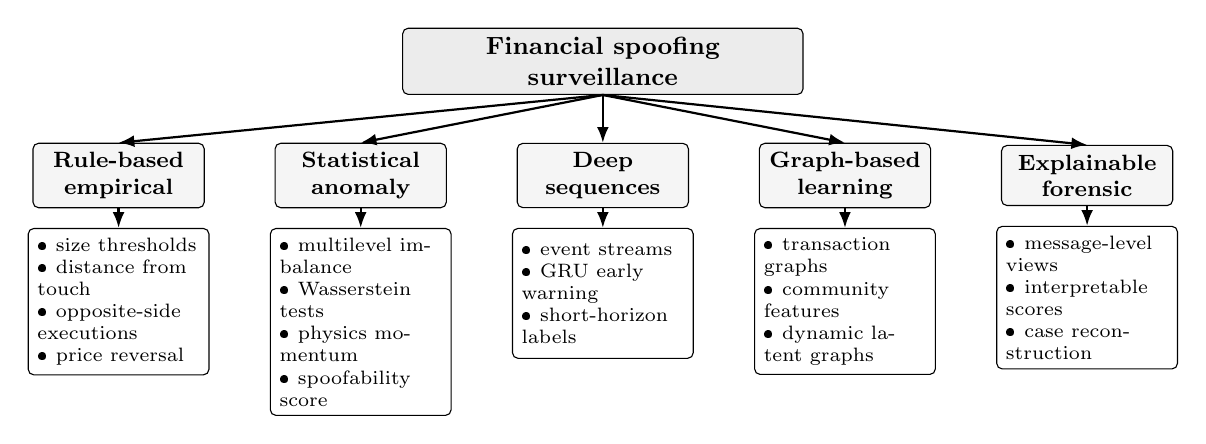
\begin{tikzpicture}[
        font=\scriptsize,
        root/.style={
            draw,
            rounded corners=2pt,
            fill=gray!15,
            align=center,
            text width=0.40\textwidth,
            minimum height=0.8cm,
            font=\small\bfseries
        },
        category/.style={
            draw,
            rounded corners=2pt,
            fill=gray!8,
            align=center,
            text width=0.16\textwidth,
            minimum height=0.75cm,
            font=\footnotesize\bfseries
        },
        detail/.style={
            draw,
            rounded corners=2pt,
            fill=white,
            align=left,
            text width=0.17\textwidth,
            minimum height=1.65cm
        },
        arrow/.style={-{Latex[length=2mm]}, thick}
    ]
        \node[root] (root) at (0,0) {Financial \mbox{spoofing} surveillance};

        \node[category] (rules) at (-6.15,-1.45) {Rule-based\\empirical};
        \node[category] (stat) at (-3.075,-1.45) {Statistical\\anomaly};
        \node[category] (seq) at (0,-1.45) {Deep\\sequences};
        \node[category] (graph) at (3.075,-1.45) {Graph-based\\learning};
        \node[category] (expl) at (6.15,-1.45) {Explainable\\forensic};

        \node[detail, below=0.25cm of rules] (rulesd) {\textbullet\ size thresholds\\\textbullet\ distance from touch\\\textbullet\ opposite-side executions\\\textbullet\ price reversal};
        \node[detail, below=0.25cm of stat] (statd) {\textbullet\ multilevel imbalance\\\textbullet\ Wasserstein tests\\\textbullet\ physics momentum\\\textbullet\ spoofability score};
        \node[detail, below=0.25cm of seq] (seqd) {\textbullet\ event streams\\\textbullet\ GRU early warning\\\textbullet\ short-horizon labels};
        \node[detail, below=0.25cm of graph] (graphd) {\textbullet\ transaction graphs\\\textbullet\ community features\\\textbullet\ dynamic latent graphs};
        \node[detail, below=0.25cm of expl] (expld) {\textbullet\ message-level views\\\textbullet\ interpretable scores\\\textbullet\ case reconstruction};

        \foreach \target in {rules,stat,seq,graph,expl} {
            \draw[arrow] (root.south) -- (\target.north);
        }
        \foreach \source/\target in {rules/rulesd,stat/statd,seq/seqd,graph/graphd,expl/expld} {
            \draw[arrow] (\source.south) -- (\target.north);
        }
    \end{tikzpicture}
    \caption{Method families in the spoofing-detection literature. The categories can overlap; each column identifies
    the main object or representation used by a strand of work.}
    \label{fig:method_taxonomy}
\end{figure}
\FloatBarrier

\section{Economic reasoning and data}
\label{sec:data}

The same cancellation can arise from different trading motives, so its interpretation depends on the surrounding sequence. This section develops the economic contrast between ordinary liquidity management and the temporary display hypothesized in spoofing. We then describe how the available messages, participant identities, and observation windows let us examine that contrast without assuming that the records reveal intent.

\subsection{What should we observe?}
\label{sec:mm_vs_spoofing}
\label{subsec:market_maker}
\label{subsec:spoofing}
A market maker offers to trade on both sides of the book. The best bid is the highest visible buying price, and the best ask is the lowest visible selling price. Their difference is the spread; their average is the midprice. A market maker seeks to earn the spread while managing inventory and the risk of trading at an unfavorable price. After buying, for example, the market maker may lower its quotes to discourage further purchases and encourage sales. Cancelling and replacing orders is part of that adjustment.

In the spoofing hypothesis, by contrast, the large displayed orders serve a directional purpose: they are intended to help a trade on the other side. For a sale, the expected sequence is large buy orders, a favorable upward price movement, the sale, and withdrawal of the buy orders. A subsequent downward movement would be consistent with the displayed pressure having been temporary. This is a hypothesis about a mechanism, not a claim that every such price movement is caused by the orders.

These explanations motivate different reference patterns for the displayed book. A market maker can adjust both sides as its inventory and exposure change, and may replace cancelled orders rather than remove liquidity altogether. The spoofing hypothesis instead suggests a large temporary display on one side, an execution on the other, and a rapid disappearance of that asymmetry afterward. Location also matters: a displayed order away from the best quote may remain visible while facing less immediate execution risk. We use these contrasts to construct the method. We do not assume that all market makers rebalance smoothly or that every spoofing attempt has the same shape.

Table~\ref{tab:surveillance-models} summarizes the economic contrast used to motivate the measurements.
\begin{table}[htbp]
\centering
\caption{Stylized differences used to construct the surveillance diagnostics. These differences describe economic
benchmarks, not observed intent or necessary conditions for either activity.}
\label{tab:surveillance-models}
\renewcommand{\arraystretch}{1.4}
\setlength{\tabcolsep}{8pt}
\rowcolors{2}{gray!4}{white}

\begin{tabularx}{\textwidth}{
    >{\raggedright\arraybackslash\bfseries}p{0.25\textwidth}
    >{\raggedright\arraybackslash}X
    >{\raggedright\arraybackslash}X
}
\toprule
\rowcolor{gray!15}
\textbf{Microstructure Feature} & \textbf{Legitimate Market Maker} & \textbf{Hypothesized Spoofing-Compatible Mechanism} \\
\midrule
Primary objective
& Earn the bid--ask spread while controlling inventory and adverse-selection risk.
& Improve a directional execution through a displayed order-book signal. \\

Order-book imbalance
& Usually maintains two-sided liquidity, with asymmetry arising from inventory and risk management.
& A large, short-lived asymmetry forms the candidate posture. \\

Cancellation motive
& Update quotes to track fair value, control inventory, or limit adverse selection.
& Withdrawal after the smaller opposite-side execution is consistent with the mechanism. \\

Posting-distance trade-off
& Quote near the touch to increase execution probability and earn the spread.
& Remain visible while reducing the risk that the displayed posture executes. \\

Source of expected gain
& Spread capture, without intentionally moving the midprice in a chosen direction.
& A potential favorable price change for the smaller order on the opposite side. \\
\bottomrule
\end{tabularx}
\end{table}

\subsection{Messages, participants, and executions}
We use CONSOB order-level messages for three equities. Ferrari covers 13 June 2024, Nexi covers 23 April 2024, and Risanamento covers June--November 2024. The samples differ in duration and composition, so differences between them cannot be attributed to the securities alone. The messages record order submissions, changes, trades, and cancellations. Replaying them lets us reconstruct the visible book and follow individual orders.

We examine the first ten occupied price levels on each side, ranked from the best quote outward. An order deeper in the book may still be visible while being less exposed to immediate execution. We therefore do not restrict the analysis to orders at the best bid or ask. The analysis concerns visible liquidity, not an estimate of all trading interest.

Actions are attributed to the original client code when it is available. When it is absent, we use the firm identifier and retain that observation level separately. A firm may represent several clients. Thus, a firm-level sequence connects the firm's recorded activity, not necessarily the decisions of one economic account. Throughout the paper, ``participant'' refers to this recorded attribution unit.

One order can trade in several partial fills. We group related fills into an \emph{execution cluster}, called an execution in the rest of the paper. The fills must share the participant, order, role, side, and trading partition. Consecutive fills must be no more than $100$ milliseconds apart, without an intervening lifecycle change for that order. A passive execution fills an order already resting in the book; an aggressive execution crosses the spread against resting orders. Passive fills share a resting price, whereas an aggressive order may execute at several prices. Appendix~\ref{sec:data_details} gives the complete grouping and identity rules.

We use $c$ for the full canonical execution identity, which fixes the instrument, trading partition, attributed participant, and execution role. Execution-bound quantities therefore omit a redundant participant index and the fixed depth $n=10$. This convention identifies recorded activity, not an economic account. Liquidity profiles suppress the participant and instrument indices locally; the execution identity restores them whenever comparisons require it. Unless stated otherwise, execution-bound sets and quantities refer to one fixed age policy; changing that policy requires reconstructing eligibility and cancellation assignment. Horizon-dependent quantities retain $H$ unless a fixed-setting convention is stated locally.

\section{Method: changes in the book around an execution}
\label{sec:model}
Throughout this section, we consider a fixed execution and its associated participant and instrument. We omit indices identifying these objects whenever no ambiguity arises. The analysis uses the first ten occupied price levels on each side of the order book. We retain the execution index $c$ when comparing executions and the horizon $H$ when changing the observation window. All order-level quantities refer to a fixed age policy unless stated otherwise.

\subsection{Economic intuition}
A participant displays liquidity, executes on the opposite side, and withdraws previously displayed orders. Under the spoofing hypothesis, the display supports the opposite-side trade before being removed. Ordinary liquidity management can produce the same sequence: a participant may withdraw exposed orders after its inventory or market conditions change. The question is therefore not simply whether cancellation follows a trade, but how substantial the removal is and what happens to the participant's remaining display.

We answer these questions with two distinct diagnostics. The withdrawal score measures the economic scale of the initial display and its removal relative to execution and available market depth. The profile diagnostic measures the largest positive change in the participant's liquidity profile shift over a short interval following execution. Following initial orders establishes gross cancellation; following the whole profile reveals whether replacement and rebalancing maintain displayed liquidity. Their joint use corroborates the reconstructed sequence without requiring the measurements to be statistically independent. These measurements are not combined into another score. Figure~\ref{fig:topn_spoofing_timeline} illustrates the sale sequence; reversing the sides gives the corresponding purchase sequence.

% The schematic is kept in the main source immediately after this subsection.
\begin{figure}[htbp]
    \centering
    \resizebox{0.95\textwidth}{!}{%
    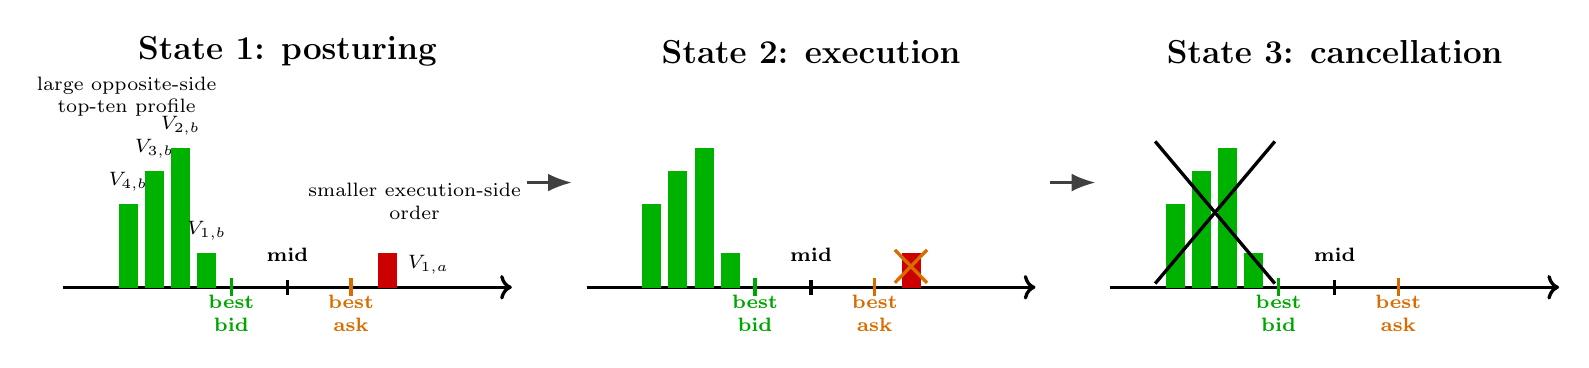
\begin{tikzpicture}[
        x=0.95cm,
        y=0.95cm,
        font=\small,
        book/.style={->, very thick},
        quote/.style={very thick},
        bid/.style={green!65!black},
        ask/.style={orange!85!black},
        fake/.style={fill=green!70!black, draw=green!70!black},
        real/.style={fill=red!80!black, draw=red!80!black},
        layer/.style={draw=black!45, fill=gray!8, rounded corners=2pt, minimum width=0.40cm},
        dist/.style={<->, black!70, very thick}
    ]
        \foreach \xshift/\step in {0/State 1: posturing,7.0/State 2: execution,14.0/State 3: cancellation} {
            \node[font=\large\bfseries] at (\xshift+3.0,3.15) {\step};
            \draw[book] (\xshift,0) -- (\xshift+6.0,0);
            \draw[quote,bid] (\xshift+2.25,-0.12) -- (\xshift+2.25,0.12)
                node[below=0.08cm, align=center, font=\scriptsize\bfseries] {best\\bid};
            \draw[quote] (\xshift+3.00,-0.10) -- (\xshift+3.00,0.10)
                node[above=0.10cm, font=\scriptsize\bfseries] {mid};
            \draw[quote,ask] (\xshift+3.85,-0.12) -- (\xshift+3.85,0.12)
                node[below=0.08cm, align=center, font=\scriptsize\bfseries] {best\\ask};
        }

        % State 1: layered bid-side deceptive profile and small ask-side bona fide order.
        \foreach \x/\h/\lab in {0.75/1.10/{$V_{4,b}$},1.10/1.55/{$V_{3,b}$},1.45/1.85/{$V_{2,b}$},1.80/0.45/{$V_{1,b}$}} {
            \draw[fake] (\x,0) rectangle +(0.24,\h);
            \node[above, font=\scriptsize] at (\x+0.12,\h+0.05) {\lab};
        }
        \draw[real] (4.22,0) rectangle +(0.24,0.45);
        \node[right, font=\scriptsize] at (4.48,0.30) {$V_{1,a}$};
        \node[align=center, font=\scriptsize] at (0.85,2.55) {large opposite-side\\top-ten profile};
        \node[align=center, font=\scriptsize] at (4.70,1.15) {smaller execution-side\\order};

        % State 2.
        \foreach \x/\h in {7.75/1.10,8.10/1.55,8.45/1.85,8.80/0.45} {
            \draw[fake] (\x,0) rectangle +(0.24,\h);
        }
        \draw[real] (11.22,0) rectangle +(0.24,0.45);
        \draw[orange!85!black, very thick] (11.12,0.06) -- (11.55,0.50);
        \draw[orange!85!black, very thick] (11.55,0.06) -- (11.12,0.50);


        % State 3.
        \foreach \x/\h in {14.75/1.10,15.10/1.55,15.45/1.85,15.80/0.45} {
            \draw[fake] (\x,0) rectangle +(0.24,\h);
        }
        \draw[black, very thick] (14.60,0.05) -- (16.20,1.95);
        \draw[black, very thick] (16.20,0.05) -- (14.60,1.95);


        \draw[-{Latex[length=3mm]}, thick, black!75] (6.2,1.4) -- (6.8,1.4);
        \draw[-{Latex[length=3mm]}, thick, black!75] (13.2,1.4) -- (13.8,1.4);
    \end{tikzpicture}%
    }
    \caption{Schematic top-ten timeline for the hypothesized spoofing mechanism. The large candidate posture forms an
    participant-specific depth profile over several bid levels, while the smaller order rests near the opposite best quote. The
    construction applies symmetrically to candidate buy- and sell-intent episodes. The figure shows the passive execution
    route; the operational reconstruction also admits an aggressive execution by the same actor.}
    \label{fig:topn_spoofing_timeline}
\end{figure}
\FloatBarrier



\subsection{The participant's liquidity profile}
\label{sec:spoofer_timeline}
\label{subsec:topn_depth_profiles}
By a liquidity profile we mean the participant's display across sides and price levels. The same quantity can represent a large presence in a thin book and a small presence in a deep one. We therefore compare participant quantity with total market depth at each occupied rank, then combine the shares using calibrated importance weights:
\begin{equation}
    \ell_s(t)=\sum_{k=1}^{10}w_{k,s}\frac{V_{k,s}(t)}{D_{k,s}(t)},
    \qquad s\in\{b,a\}.
    \label{eq:weighted_topn_liquidity}
\end{equation}
Here $V_{k,s}(t)$ is the participant's displayed quantity at rank $k$ on side $s$, $D_{k,s}(t)$ is total displayed market depth at that rank and side, and $w_{k,s}$ is its nonnegative calibrated weight. Rank one is the best quote; $b$ denotes bid and $a$ ask. A zero-depth level contributes zero, as specified in Appendix~\ref{sec:depth_calibration}; missing inputs are not made valid by that convention. Weights sum to one separately on each side and remain fixed within each instrument.

The weights reflect the trade-off between visibility and fill probability that motivates the hypothesized display. Under the spoofing hypothesis, an order must be visible to other participants while remaining unlikely to execute. We represent visibility through the strength of the association between a level's relative market depth and subsequent midprice movements. We represent exposure to execution by how often subsequent trades reach that level's snapshot price. A level receives greater weight when its price association is stronger and its price is less frequently reached. These are descriptive proxies: visibility is not a direct measurement of attention or causal price impact, and price-reaching frequency is not the fill probability of an individual order, which also depends on queue position and intervening events.

The calibrated weights differ across ranks, book sides, and instruments. Table~\ref{tab:empirical_depth_kernel_calibration} retains the side-specific estimates used in the calculations. Figure~\ref{fig:empirical_top10_kernel_profiles} summarizes their arithmetic average across sides for visualization; Figures~\ref{fig:empirical_topn_visibility_profiles} and~\ref{fig:empirical_topn_execution_risk_profiles} show the visibility proxy and price-reaching frequencies underlying the trade-off. Calibration uses $H_{\mathrm{cal}}=1$ second throughout, including when participant behavior is followed for longer. Appendix~\ref{sec:depth_calibration} gives the estimation procedure, normalization, and uncertainty calculations. The weights use the full sample of each instrument; prospective evaluation would require estimation on earlier data.

\begin{table}[htbp]
\centering
\caption{Full-sample empirical top-$10$ depth-kernel weights recalibrated at horizon $H_{\mathrm{cal}}=1$ second. Values are rounded to
three decimal places and sum to one within each instrument and side before rounding.}
\label{tab:empirical_depth_kernel_calibration}
\small
\setlength{\tabcolsep}{3pt}
\begin{tabular}{ll*{10}{r}}
\toprule
Instrument & Side & $\widehat w_1$ & $\widehat w_2$ & $\widehat w_3$ & $\widehat w_4$ & $\widehat w_5$ & $\widehat w_6$ & $\widehat w_7$ & $\widehat w_8$ & $\widehat w_9$ & $\widehat w_{10}$ \\
\midrule
Risanamento & Ask & 0.108 & 0.263 & 0.362 & 0.011 & 0.016 & 0.043 & 0.000 & 0.019 & 0.104 & 0.073 \\
 & Bid & 0.645 & 0.036 & 0.024 & 0.148 & 0.053 & 0.023 & 0.019 & 0.037 & 0.014 & 0.002 \\
Nexi & Ask & 0.103 & 0.023 & 0.021 & 0.177 & 0.253 & 0.052 & 0.315 & 0.019 & 0.006 & 0.032 \\
 & Bid & 0.073 & 0.131 & 0.104 & 0.208 & 0.223 & 0.120 & 0.028 & 0.030 & 0.004 & 0.078 \\
Ferrari & Ask & 0.060 & 0.040 & 0.053 & 0.277 & 0.349 & 0.023 & 0.163 & 0.012 & 0.002 & 0.022 \\
 & Bid & 0.154 & 0.095 & 0.023 & 0.103 & 0.116 & 0.248 & 0.005 & 0.071 & 0.114 & 0.070 \\
\bottomrule
\end{tabular}
\end{table}

\input{generated/simple_notation_20261020/kernel_figures.tex}
\FloatBarrier

To distinguish ask-dominated from bid-dominated display, we use the liquidity imbalance:
\begin{equation}
    I(t)=\begin{cases}
        \dfrac{\ell_a(t)-\ell_b(t)}{\ell_a(t)+\ell_b(t)},
            &\ell_a(t)+\ell_b(t)>0,\\[4pt]
        \text{undefined},&\ell_a(t)+\ell_b(t)=0.
    \end{cases}
    \label{eq:multilevel_dwi}
\end{equation}
When defined, $I$ lies in $[-1,1]$. Positive values indicate ask-side dominance and negative values bid-side dominance. Values near zero indicate approximately balanced weighted shares only when liquidity is present. The reconstructed series records zero once to mark disappearance of a previously observed profile; other undefined values remain missing. That marker is not evidence of renewed balance. Figure~\ref{fig:topn_imbalance_dynamics} illustrates the economic contrast, not an empirical classification rule.

\begin{figure}[htbp]
    \centering
    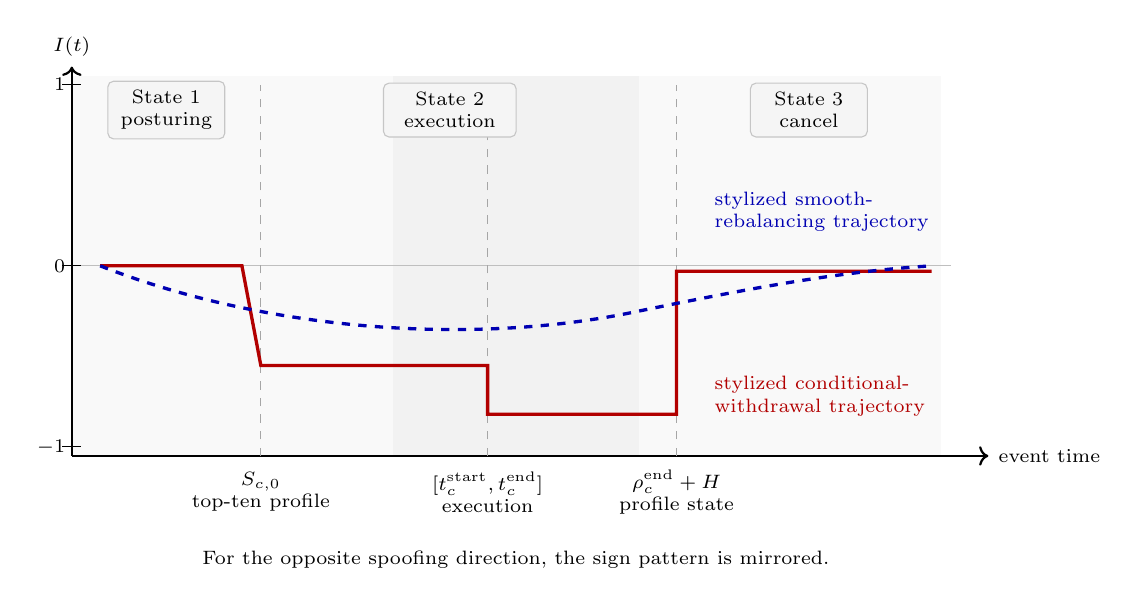
\begin{tikzpicture}[
        x=2.4cm,
        y=2.3cm,
        font=\scriptsize,
        axis/.style={->, thick},
        spoof/.style={very thick, red!70!black},
        maker/.style={very thick, dashed, blue!70!black},
        event/.style={gray!70, dashed},
        state/.style={fill=gray!8, draw=gray!45, rounded corners=2pt, align=center}
    ]
        \fill[gray!5] (0,-1.05) rectangle (1.7,1.05);
        \fill[gray!10] (1.7,-1.05) rectangle (3.0,1.05);
        \fill[gray!5] (3.0,-1.05) rectangle (4.6,1.05);

        \draw[axis] (0,-1.05) -- (0,1.1) node[above] {$I(t)$};
        \draw[axis] (0,-1.05) -- (4.85,-1.05) node[right] {event time};
        \draw[gray!50] (-0.05,0) -- (4.65,0);

        \foreach \y/\lab in {-1/$-1$,0/$0$,1/$1$} {
            \draw (-0.05,\y) -- (0.05,\y) node[left=0.08cm] {\lab};
        }

        \draw[event] (1.0,-1.05) -- (1.0,1.0);
        \draw[event] (2.2,-1.05) -- (2.2,1.0);
        \draw[event] (3.2,-1.05) -- (3.2,1.0);

        \node[state, text width=1.25cm] at (0.5,0.86) {State 1\\posturing};
        \node[state, text width=1.45cm] at (2.0,0.86) {State 2\\execution};
        \node[state, text width=1.25cm] at (3.9,0.86) {State 3\\cancel};

        \node[align=center] at (1.0,-1.25) {$S_{c,0}$\\top-ten profile};
        \node[align=center] at (2.2,-1.25) {$[t_c^{\mathrm{start}},t_c^{\mathrm{end}}]$\\execution};
        \node[align=center] at (3.2,-1.25) {$\rho_c^{\mathrm{end}}+H$\\profile state};

        \draw[spoof] (0.15,0) -- (0.9,0)
            -- (1.0,-0.55) -- (2.2,-0.55)
            -- (2.2,-0.82) -- (3.2,-0.82)
            -- (3.2,-0.03) -- (4.55,-0.03);

        \draw[maker] (0.15,0) .. controls (1.0,-0.35) and (2.1,-0.45) .. (3.0,-0.25)
            .. controls (3.7,-0.10) and (4.1,-0.03) .. (4.55,0);

        \node[red!70!black, align=left, anchor=west] at (3.35,-0.72) {stylized conditional-\\withdrawal trajectory};
        \node[blue!70!black, align=left, anchor=west] at (3.35,0.30) {stylized smooth-\\rebalancing trajectory};
        \node[align=center] at (2.35,-1.62) {For the opposite spoofing direction, the sign pattern is mirrored.};
    \end{tikzpicture}
    \caption{Stylized execution-time behavior of the liquidity imbalance. The conditional-withdrawal
    trajectory shows a large top-ten imbalance returning rapidly toward zero after the opposite-side execution. The smooth
    trajectory illustrates gradual rebalancing. Neither trajectory is an empirical classification rule.}
    \label{fig:topn_imbalance_dynamics}
\end{figure}
\FloatBarrier



\subsection{Changes in the liquidity profile}
\label{subsec:multilevel_conditionality}
\label{subsec:msci_grid_method}
An imbalance change alone does not identify which side recedes. For a sale, withdrawal of the hypothesized display occurs on the bid side; for a purchase, it occurs on the ask side. Let $s$ denote the execution side and $\bar s$ its opposite. We measure each side's proportional reduction from its pre-execution weighted share:
\begin{equation}
    r_s(H)=\begin{cases}
        \dfrac{[\ell_s(t_c^-)-\ell_s(t_c^+)]_+}{\ell_s(t_c^-)},
            &\ell_s(t_c^-)>0,\\[4pt]
        0,&\ell_s(t_c^-)=0.
    \end{cases}
    \label{eq:side_collapse}
\end{equation}
Here $[x]_+=\max\{x,0\}$. The state $t_c^-$ is the last retained participant state before the first execution message. The state $t_c^+$ depends on $H$: it is the last supported retained state at or before $H$ seconds after the final execution message's sequence time. These labels identify selected book states, not new trade timestamps. Missing required states leave profile changes missing. Appendix~\ref{sec:profile_technical} specifies observation support and evaluation of the zero-initial-liquidity branch.

A directional profile shift combines the magnitude of imbalance change with the difference between the two reductions:
\begin{equation}
    \Phi_c(H)=\frac12\left|I(t_c^+)-I(t_c^-)\right|
                 +r_{\bar s}(H)-r_s(H).
    \label{eq:signed_msci}
\end{equation}
The first component measures imbalance change, scaled to $[0,1]$; the second increases the shift when opposite-side liquidity recedes; the third offsets execution-side recession. The shift lies in $[-1,2]$ when defined, without clipping. It is an intermediate description of profile change, not another ranking score. Fills, replacement orders, changes in rank, and other participants' depth can change the weighted shares without cancellation of the initial orders.

To locate a sharp transition rather than only an endpoint difference, we evaluate the same shift throughout the window, always keeping the pre-execution baseline fixed. Its largest positive increment over a 50-millisecond interval is
\begin{equation}
    J_c(H)=\max_k\left[\Phi_c(u_k)-\Phi_c(u_{k-\lambda})\right]_+.
    \label{eq:msci_grid_increment}
\end{equation}
The elapsed-time grid has 10-millisecond spacing, includes both endpoints of $[0,H]$, and compares nodes five steps apart ($\lambda=5$). Here $\Phi_c(u)$ evaluates the shift at elapsed sequence time $u$, always against the same pre-execution profile. We use $H\in\{1,2,5,10\}$ seconds, with ten seconds primary. The complete grid definition, canonical message ordering, forward carry of retained states, missing-profile rules, and maximizing-interval ties are in Appendix~\ref{sec:profile_technical}.

A large $J$ indicates a sharp positive profile-shift change, not spoofing or speed independently of amplitude. A persistent and a temporary increase can have the same $J$; a constant trajectory has $J=0$, but $J=0$ does not imply an unchanged profile. Incomplete trajectories remain missing rather than zero. The profile includes every displayed order at the first ten levels, irrespective of age, so $J$ does not change across age policies for a fixed execution and horizon. It neither selects candidates nor determines the withdrawal-score ranking.

\subsection{Withdrawal and market relevance}
\label{subsec:withdrawal_market_age}
To establish actual withdrawal, we fix the participant's opposite-side orders present within the first ten market levels immediately before execution. Their initial quantity is $P_c$; later submissions do not enter this display. The execution quantity is $Q_c>0$, and $U_c(H)$ is the physical quantity withdrawn through assigned cancellations within the horizon. Finally, $D_c$ is total opposite-side market depth over those ten levels in the exact pre-execution book, including the participant's orders. This denominator stays fixed rather than following later market depth.

The ratios $U_c(H)/Q_c$ and $U_c(H)/P_c$ answer different questions: how much is withdrawn relative to execution, and how much of the initial display disappears? The latter lies in $[0,1]$ when $P_c>0$ and is undefined when $P_c=0$. No assigned cancellation gives $U_c(H)=0$. Withdrawal is gross removal: replacement orders are not subtracted. Initial-order caps prevent repeated cancellations or later size increases from inflating removal, and assignment is exclusive within each horizon and age setting. Appendix~\ref{sec:withdrawal_technical} gives the complete physical accounting.

Observation of withdrawal starts from the final execution trade time, whereas profile observation starts from its final message's sequence time. Withdrawal includes nonnegative cancellation delays strictly below $H$ and requires source-order precedence. These clocks have an operationally assumed common origin, not independently certified synchronization; all comparisons retain integer nanoseconds (Appendix~\ref{sec:data_details}).

An older visible order remains eligible in the main specification, but receives less weight in the score. For initial order age $a$, the main weight is
\begin{equation}
    g(a)=2^{-a/(30\,\mathrm{s})}.
    \label{eq:shared_order_age_weight}
\end{equation}
The weight halves every 30 seconds. Age is measured from the lifecycle's first observed sequence time to the first execution message and frozen there. The same frozen weight multiplies the initial displayed quantity and its subsequent counted cancellation, giving $P_c^{\mathrm{age}}$ and $U_c^{\mathrm{age}}(H)$. Only initial order age is discounted: there is no cancellation-delay discount. Neither $Q_c$, $D_c$, nor the complete liquidity profile is age-discounted. The 30-second half-life is an exploratory specification, not a fitted behavioral constant. Full sums, lifecycle conventions, and alternative policies are given in Appendix~\ref{sec:withdrawal_technical}.

We measure the economic scale of withdrawal with the withdrawal score:
\begin{equation}
    W_c(H)=
      \log\!\left(1+\frac{P_c^{\mathrm{age}}}{Q_c}\right)
      \log\!\left(1+\frac{U_c^{\mathrm{age}}(H)}{Q_c}\right)
      \frac{U_c^{\mathrm{age}}(H)}{D_c}.
    \label{eq:wmsci_market_age}
\end{equation}
Here $\log$ is the natural logarithm. The first factor describes initial display relative to execution; the second describes withdrawal relative to execution. Their logarithms moderate very large quantity ratios. The third factor places withdrawal relative to initial market depth. It remains linear so that, holding the logarithmic factors fixed, the score is proportional to the market share withdrawn. Multiplication emphasizes their joint presence: a small component attenuates the others, and no withdrawal gives zero. An additive score could reward display without removal unless another rule prevented it.

The score is nonnegative and has no fixed upper bound. It orders review, not manipulation probabilities. Accounting ensures $0\leq U_c^{\mathrm{age}}(H)\leq P_c^{\mathrm{age}}\leq D_c$ when depth is measured, so its final factor lies in $[0,1]$. For $Q_c>0$ and positive measured $D_c$, zero weighted display or withdrawal gives $W=0$ directly. Missing or zero $D_c$ makes the score unavailable; no artificial denominator quantity is added. Underflow of age weights or scores never removes a physical candidate. The score uses aggregate top-ten quantity, while $J$ describes rapid change in the relative profile; neither replaces the other.

\subsection{Candidate identification and review ranking}
\label{subsec:candidature_priority}
An execution is a candidate in a horizon and age setting precisely when executed quantity, eligible raw initial display, and assigned raw withdrawal are all positive. No minimum withdrawal-to-execution ratio, profile threshold, score threshold, or favorable-price condition is imposed. Every execution and parameter setting remains represented, including non-candidates, so changes in coverage can be traced.

Within each instrument and setting, candidates with finite scores are ordered by descending $W$, including zero scores at the end. Ties use stable execution identifiers, then partition and participant identifiers. Candidates without finite scores remain explicitly unranked, with a reason; missing scores are not replaced by zero. The analyst's stopping depth is a workload decision, not a boundary between manipulation and legitimate activity.

The value of $J$ accompanies the execution without filtering, reordering, or breaking ties. A small $J$ can coexist with substantial removal, and a large $J$ can precede cancellation of the initial display. Price diagnostics likewise add interpretation without changing membership or rank. Comparisons across settings retain the original execution identity: repeated views and shared physical messages are not independent evidence. Appendix~\ref{subsec:event_reconstruction} defines shared-order episodes as a contextual grouping, not another selection.

\subsection{Price diagnostics}
\label{sec:price_measures_simple}
\label{subsec:primary_price_selection}
\label{sec:joint_selection_simple}
The hypothesized purpose of the display is to improve an opposite-side trade. Prices therefore ask three additional questions: does the midprice move favorably before execution, does it revert after withdrawal, and how does the actual execution price compare with the completed display? These comparisons retain source price units, not ticks, and do not identify causal price effects.

Let $M(t)$ be the midprice and let $d_c=+1$ for a sale and $d_c=-1$ for a purchase, so favorable movement is positive. The completed-display benchmark $S_{c,0}$ is the saved state immediately after the last candidate order was first observed in source order. It must strictly precede the execution's first message; it is not the price before all orders were placed. Favorable price movement is
\begin{equation}
    \operatorname{FPM}_c=d_c\left[M(t_c^-)-M(S_{c,0})\right].
    \label{eq:favorable_price_move}
\end{equation}
A higher pre-execution midprice is favorable to a sale, and a lower one to a purchase. The saved state $t_c^-$ need not be the immediately adjacent global book. Missing benchmarks remain missing rather than zero.

Reversion checks the opposite direction after assigned cancellations. For each positive counted cancellation $j$, let $M_j^{\mathrm{saved}}$ be the last retained pre-cancellation midprice and $M_j^{R}$ the retained price at or before $\rho_j+H_R$, with the separate reversion horizon $H_R=2$ seconds. Using physical counted quantities $\bar q_{c,j}$, we define
\begin{equation}
    \operatorname{REV}_c=
    \frac{\sum_{j\in\mathcal C_c^+(H)}\bar q_{c,j}d_c
                [M_j^{\mathrm{saved}}-M_j^{R}]}
         {\sum_{j\in\mathcal C_c^+(H)}\bar q_{c,j}}.
    \label{eq:price_reversion}
\end{equation}
Here $\mathcal C_c^+(H)$ contains all assigned cancellations with positive counted quantity. The value is defined only when this set is nonempty and every member has both finite prices and supported observation through its target. Otherwise complete REV is missing; an observed-subset mean does not replace it. The weights are physical quantities, not age weights or cancellation-delay discounts. The retained market quotes need not be fresh at two seconds, and no maximum saved-state age is imposed. Appendix~\ref{subsec:price_response_diagnostics} specifies joins, equal-time ordering, and missing-price rules.

Finally, let $\bar p_c$ be the quantity-weighted execution price. Execution advantage is
\begin{equation}
    \operatorname{ADV}_c=d_c\left[\bar p_c-M(S_{c,0})\right].
    \label{eq:execution_advantage}
\end{equation}
Positive ADV means selling above or buying below the completed-display midprice. It is a price comparison, not realized profit, and can reflect the spread even without favorable midprice movement. Subtracting FPM gives the signed difference between execution price and the saved pre-execution midprice.

The reported prices use the main ten-second withdrawal window and 30-second age half-life; these setting arguments are suppressed in FPM, REV, and ADV. Every one of the 6,914 candidates remains in its instrument's denominator, including zero-score candidates and positive, zero, negative, or missing prices. Values within the endpoint-scale floating-point bound count as numerical zero only for sign summaries and medians, without changing raw prices or selection. Appendix~\ref{subsec:price_numerical_signs} gives this convention and its sensitivity check. Appendix~\ref{subsec:price_response_diagnostics} also retains the alternative microprice and the accounting decomposition of observed reversion, not a counterfactual market without the participant.

Table~\ref{tab:simple-terminology} collects the observational units and the distinct roles of candidature and review priority.
\begin{table}[!htbp]
\centering
\caption{Terms used in the main specification. Candidate orders need not be cancelled, whereas a candidate execution requires positive assigned withdrawal. Executions, not orders or episodes, are the unit of the main comparisons.}
\label{tab:simple-terminology}
\begin{singlespace}
\renewcommand{\arraystretch}{1.18}
\begin{tabularx}{\textwidth}{@{}>{\raggedright\arraybackslash}p{0.25\textwidth}>{\raggedright\arraybackslash}X@{}}
\toprule
Term & Meaning in this paper \\
\midrule
Message or fill & An individual source record. Related partial fills can be grouped into one execution. \\
Execution (execution cluster) & Fills of the same order grouped under the participant, role, side, partition, lifecycle, price, and time-gap rules. Called an execution after its definition. \\
Participant & The original client where identified, or a separately retained firm fallback. Firm fallback can pool several clients; it is not the complete intermediary view below. \\
Candidate orders or initial display & The participant's opposite-side orders active within the first ten market price levels immediately before execution. The main setting retains all observable nonnegative ages; later orders do not enter this display. \\
Assigned withdrawal & Cancellation of initial orders assigned exclusively to an execution within the observation window and capped at their initial quantity. This is gross removal, without subtracting replacements. \\
Candidate execution & An execution with positive executed quantity, eligible raw initial display, and assigned raw withdrawal in the stated setting. No $W$, profile, or price-sign threshold is required. \\
Withdrawal-score rank & The position obtained by ordering candidates by decreasing withdrawal score within instrument and setting. Finite zero scores remain; unavailable scores are explicitly unranked. \\
Profile diagnostic $J$ & The largest positive profile-shift increment over the specified short comparison interval. It accompanies the ranking without selecting candidates or changing their order. \\
Shared-order episode & Executions connected, directly or indirectly, through shared candidate-order lifecycles within participant, execution side, partition, and recorded date. This grouping supplies context, not a further selection. \\
Identified-client and intermediary views & Client groups use executions with an identified client. Intermediary groups use the original firm on every execution, including client-identified and firm-only activity. The views overlap and are not additive. \\
\bottomrule
\end{tabularx}
\end{singlespace}
\end{table}
\FloatBarrier


\FloatBarrier


\section{Results}
\label{sec:results}

The main specification retains older visible orders while giving recent display greater weight. Extending observation reveals later cancellations, and $W$ places their importance on a market scale when ordering review. Prices across the full candidate population show which parts of the proposed economic sequence are observed. Grouping executions by identified client and intermediary then establishes how concentrated the reconstructed activity is.

Figure~\ref{fig:results_selection_map} separates construction of the candidate population from its review order.

\begin{figure}[!htbp]
    \centering
    \begin{singlespace}
    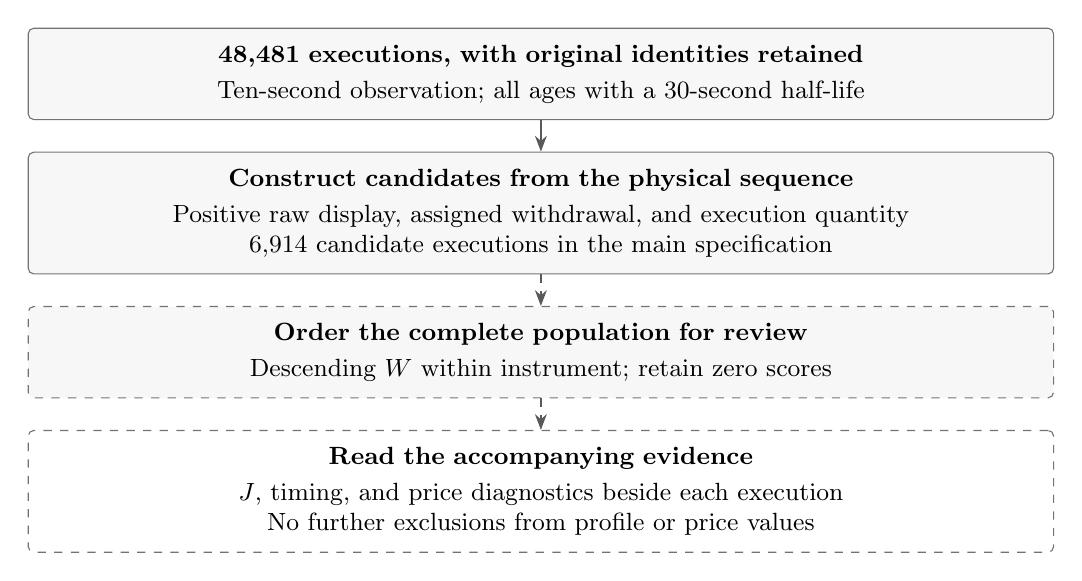
\begin{tikzpicture}[
        font=\small,
        roadmapbox/.style={draw=black!55, rounded corners=2pt, align=center,
            inner sep=6pt, text width=12.6cm, fill=black!3},
        roadmaparrow/.style={-{Stealth[length=2mm]}, thick, draw=black!65}
    ]
        \node[roadmapbox] (all) {\textbf{48,481 executions, with original identities retained}\\[2pt]
            Ten-second observation; all ages with a 30-second half-life};
        \node[roadmapbox, below=4mm of all] (positive) {\textbf{Construct candidates from the physical sequence}\\[2pt]
            Positive raw display, assigned withdrawal, and execution quantity\\
            6,914 candidate executions in the main specification};
        \node[roadmapbox, dashed, below=4mm of positive] (ranked) {\textbf{Order the complete population for review}\\[2pt]
            Descending $W$ within instrument; retain zero scores};
        \node[roadmapbox, dashed, fill=white, below=4mm of ranked] (prices) {\textbf{Read the accompanying evidence}\\[2pt]
            $J$, timing, and price diagnostics beside each execution\\
            No further exclusions from profile or price values};
        \draw[roadmaparrow] (all.south) -- (positive.north);
        \foreach \source/\target in {positive/ranked,ranked/prices} {
            \draw[roadmaparrow,dashed] (\source.south) -- (\target.north);
        }
    \end{tikzpicture}
    \end{singlespace}
    \caption{Candidate construction and review order in the main specification ($H=10$ seconds, age half-life $30$ seconds, no age cap). The solid arrow constructs the physical sequence. Dashed arrows order its inspection and add diagnostic information without removing candidates. $W$ is ranked within instrument; $J$ does not filter or reorder it. Prices are evaluated for the full candidate population, with zero, negative, and missing outcomes retained. Unsupported scores, if any, remain explicitly unranked.}
    \label{fig:results_selection_map}
\end{figure}
\FloatBarrier

\subsection{Coverage depends on what we observe}
\label{subsec:observation_attribution_results}
\label{subsec:continuous_withdrawal_results}
\label{subsec:cross_instrument_results}
\label{subsec:risanamento_results}
\label{subsec:nexi_results}
\label{subsec:ferrari_results}

The reconstruction preserves 48,481 executions and their 65,471 original fills. With ten-second observation and a 30-second age half-life, 3,526 executions in Ferrari, 2,393 in Nexi, and 995 in Risanamento satisfy the raw candidate rule: 6,914 in total (Appendix Table~\ref{tab:wmsci-j-population}).



Observation time affects whether removal is recorded. Holding the main age kernel fixed, the candidate counts at one second are 2,665 in Ferrari, 1,835 in Nexi, and 545 in Risanamento. Extending observation to ten seconds increases them to the counts above. Figure~\ref{fig:multiscale-coverage} shows the intermediate horizons. Since the kernel changes scores rather than raw membership, these curves describe the timing of assigned physical removal, not a decay in the quantity displayed. The supplementary age comparisons distinguish that timing effect from exclusion by a hard age limit (Table~\ref{tab:multiscale-age-policies}).

The increase is especially pronounced in Risanamento: assigned removal for many retained displays falls after the first second. This is a finding about what the reconstruction observes, not evidence that the additional cases are more suspicious. Ferrari and Nexi each cover one day, whereas Risanamento spans several months. Coverage differences therefore remain descriptive. Exclusive cancellation assignment is evaluated at each horizon, so the union across horizons is not necessarily the longest-horizon population; the appendix keeps those quantities separate.

\begin{figure}[!htbp]
    \centering
    \includegraphics[width=\textwidth]{generated/simple_notation_20261020/coverage.pdf}
    \caption{Candidate executions by instrument at four observation horizons, with all observable ages and a 30-second exponential half-life. Counts use a common scale. Membership uses positive raw display, assigned withdrawal, and execution quantity; age weights enter scores, not these counts. Lines connect parameter settings, not an event-time trajectory. Sample coverage differs across instruments, so counts are descriptive rather than prevalence estimates.}
    \label{fig:multiscale-coverage}
\end{figure}

\FloatBarrier
All primary candidates have finite $W$ and complete finite $J$ values. Zero scores and zero rapid increments remain in the candidate population, without exclusions or changes to the ranking rule. Appendix Table~\ref{tab:rank-summary} reports their distributions and zero counts.

\subsection{Prices support different parts of the proposed sequence}
\label{subsec:behavior_price_results}

Jointly favorable movement and complete reversion are observed for 397 of 3,526 Ferrari candidates (11.3\%), 308 of 2,393 Nexi candidates (12.9\%), and 44 of 995 Risanamento candidates (4.4\%). Requiring nonnegative execution advantage as well retains 387, 273, and 38 candidates, respectively: 11.0\%, 11.4\%, and 3.8\% of the same full denominators. The comparison covers all 6,914 candidates, including the 17 Risanamento executions with numerically zero $W$, and does not require $J$ to be positive. These joint price features accompany a subset of the reconstructed sequences; they are not guaranteed by a large withdrawal score or rapid profile change.

Figure~\ref{fig:price-evidence} separates favorable, zero, adverse, and missing price outcomes while keeping the full candidate denominator. Appendix Table~\ref{tab:candidate-prices} retains the exact counts. Jointly positive movement and complete reversion identify the executions for which both measured parts of the proposed price sequence are present. This describes the evidence available beside the ranking; it does not establish that higher-ranked executions have better price corroboration or that a profile-based filter improves discrimination.




\begin{figure}[!htbp]
    \centering
    \includegraphics[width=\textwidth]{generated/simple_notation_20261020/price_evidence.pdf}
    \caption{Price evidence for all 6,914 primary candidates, including zero $W$. Left: vertical stacked bars show favorable price movement (FPM), complete two-second reversion (REV), and execution advantage relative to the completed-display benchmark (ADV). Positive, zero, negative, and missing outcomes use the full instrument-specific candidate denominator. Hatching denotes missing FPM or ADV, or missing/incomplete REV, not zero. Right: the conjunction FPM $>0$, complete REV $>0$, and ADV $\geq0$, with count/full candidate denominator above each bar. Numerical-zero ADV is included; missing ADV is not. The panels use different percentage scales. ADV compares prices, not realized profit; marginal bars do not identify joint outcomes.}
    \label{fig:price-evidence}
\end{figure}
\FloatBarrier

Neither price sign determines candidature or review rank. Among finite observations, the median favorable movement and median complete reversion are zero in each instrument. Favorable movement and execution advantage are missing for 95 candidates: 14 in Ferrari, nine in Nexi, and 72 in Risanamento. Complete reversion is missing for 25 candidates: six, three, and sixteen, respectively. A candidate with incomplete reversion is not replaced by its observed-subset average, and a missing favorable-movement benchmark is not assigned zero. These distinctions keep lack of observation separate from an observed price path that does not support the hypothesized sequence.


The ADV bars in Figure~\ref{fig:price-evidence} distinguish the execution price from the movement of the midprice. An execution price can be better than the completed-display midprice without the midprice moving favorably, because the spread also matters. Nonnegative ADV adds a separate requirement to the joint comparison: the execution price must be no worse than the completed-display benchmark under the numerical-zero convention. Missing ADV does not satisfy this requirement. This comparison does not change candidature or review rank. Appendix Table~\ref{tab:candidate-advantage} retains all advantage signs and missing observations for the same full population. The comparison is relative to the saved completed-display benchmark, not realized profit. Prices thus complement the order-level reconstruction rather than supply an automatic exclusion rule.

\FloatBarrier
\subsection{Roles and attribution}
\label{subsec:timing_recurrence_results}

The main candidate population contains both passive and aggressive executions and both original-client and firm attribution. Appendix Table~\ref{tab:multiscale-composition} reports each stratum against its execution denominator rather than pooling the roles. Firm attribution accounts for much of the candidate coverage, especially in the two single-day samples. These records connect a firm's activity and can include several clients; they should not be interpreted as decisions by one economic account.



An execution can lack assigned withdrawal in a short window, or it can be a candidate placed low in the $W$ ranking. Only the former concerns physical eligibility. Keeping role, attribution level, and candidature explicit makes that distinction inspectable without treating every record as an independent economic account. Appendix Table~\ref{tab:candidate-price-strata} separates the full candidate denominators and joint price evidence by role and attribution. Differences in pooled price summaries can reflect this composition; they do not establish a role-specific behavioral mechanism.

\FloatBarrier
\subsection{From individual executions to clients and intermediaries}
\label{subsec:participant_group_results}

Execution counts can reflect repeated activity by the same participant rather than many distinct participants. We therefore group the main-specification results in two ways: by identified client and by the intermediary carrying the execution. Client groups retain the original client identity used in reconstruction. Intermediary groups use the original firm identifier for every execution, including identified-client activity as well as firm-only activity. The two views overlap and must not be added together. A firm-only record is not assigned to an invented client.

Each group is compared with its own observed execution activity. The candidate fraction divides its candidate executions by all its executions in that instrument; it is not a manipulation rate. $W$ and $J$ are summarized over the group's candidates without adding execution scores into a participant score. The grouping preserves the original within-instrument execution ranking and includes zero-score and missing-price candidates. Repeated executions can share a display or nearby market conditions, so their number measures recurrence, not independent evidence.

Candidate executions are concentrated among a small part of the identified-client population. Ferrari has seven clients with candidates out of 323 observed clients; Nexi has nine out of 587, and Risanamento has seventeen out of 1,041. Within these identified-client candidates, the largest client contributes 293 of 355 in Ferrari (82.5\%), 385 of 496 in Nexi (77.6\%), and 264 of 403 in Risanamento (65.5\%). Five, seven, and nine clients, respectively, have at least two candidate executions. This recurrence identifies where an account-level review can examine a sequence of decisions rather than isolated executions.

The intermediary view covers all executions, including those without a usable client code. Candidates occur through twenty of 49 observed intermediaries in Ferrari, nineteen of 48 in Nexi, and eleven of 35 in Risanamento. The largest intermediary contributes 702 of 3,526 candidates in Ferrari, 385 of 2,393 in Nexi, and 316 of 995 in Risanamento (Appendix Table~\ref{tab:participant-summary}). These totals describe the activity carried through each intermediary, not a claim that the intermediary or its clients acted jointly.



The cumulative curves in Figure~\ref{fig:participant-concentration} show how much of this activity is accounted for by the most frequent entities. Within each instrument and view, entities are ordered by decreasing number of candidate executions, not by $W$. At rank $k$, the vertical coordinate is the percentage of that view's candidate executions contributed by its first $k$ entities. The marker at rank one therefore gives the largest entity's share. For example, the first Ferrari client accounts for 82.5\% of the 355 candidates attributed to identified clients; this is not the percentage of that client's executions that are candidates.

The left panel includes only identified-client activity, whereas the right panel groups all activity by intermediary. Their candidate denominators consequently differ: 355, 496, and 403 on the left, compared with 3,526, 2,393, and 995 on the right for Ferrari, Nexi, and Risanamento. The lower initial shares for intermediaries therefore do not contradict the client concentration: the right panel includes firm-only activity absent from the left. In the intermediary view, the first three entities account for 49.0\%, 46.3\%, and 84.9\% of candidates, respectively. Risanamento's candidates are thus concentrated among relatively few intermediaries as well as identified clients.

The logarithmic horizontal axis makes both the first ranks and the many entities without candidates visible. Legend entries report entities with at least one candidate over all observed entities. Each curve reaches 100\% once every entity with candidates has been included, then remains flat as zero-candidate entities are added. This concentration motivates reviewing repeated sequences at participant level, but it does not establish a higher propensity to generate candidates: that comparison requires each entity's own execution denominator, rather than its share of all candidates. Repetition also does not supply independent corroboration of manipulation.


\begin{figure}[!htbp]
    \centering
    \includegraphics[width=\textwidth]{generated/simple_notation_20261020/participant_concentration.pdf}
    \caption{Candidate executions are concentrated, especially among identified clients. Each curve cumulates candidate executions after ordering entities by decreasing candidate count within instrument and view (stable alias ties), not by $W$ or severity. Markers indicate the largest entity. All observed entities remain on the logarithmic rank axis, including zero-candidate groups on the final plateau. Legend counts give entities with candidates/all observed entities. Candidate-share denominators are 355, 496, and 403 for identified clients and 3,526, 2,393, and 995 for intermediaries (Ferrari, Nexi, Risanamento). The overlapping views must not be added. The vertical scale is common; horizontal ranges differ. These are descriptive activity shares, not independent corroboration or manipulation rates.}
    \label{fig:participant-concentration}
\end{figure}

The detailed client and intermediary tables in Appendix~\ref{subsec:participant_group_details} retain report-local labels that are consistent across instruments. They show how often the sequence recurs, its $W$ scale, the accompanying profile change, and joint price evidence. Intermediary totals may pool several clients and unidentified accounts; they do not describe the decisions of a single economic account. These summaries locate activity for further inspection, rather than establish intent or compare participant performance across samples with different coverage.

\FloatBarrier
\subsection{Scope of the empirical comparison}
\label{subsec:withdrawal_sensitivity_results}

The main specification fixes a 30-second half-life and ten-second observation. Shorter horizons and supplementary age treatments preserve execution identities, depth weights, the profile formula, and the rule for ordering candidates. They expose sensitivity to observation and recency, but do not establish an optimal horizon or half-life. The choices remain exploratory on the inspected samples. The ranking has no model-defined review cutoff and is not calibrated against a false-positive target. Grid resolution, comparison lag, book depth, fill-grouping gap, and alternative assignment rules have not been varied.

Profile support comes from the represented message sequences, not independently certified exchange-feed completeness. Timing retains the operational common-origin assumption for trade and sequence clocks. Prices describe every primary candidate, not every parameter setting. Their retained participant states need not supply fresh global quotes at the target times. These limits leave the structural findings intact: the observed display, assigned cancellations, market scale, profile transitions, and associated prices can be inspected without treating every parameter view as new evidence.

\section{Discussion and Conclusion}
\label{sec:discussion_conclusion}

Distinguishing possible spoofing from ordinary liquidity management is a surveillance problem because both can produce large visible orders followed by rapid cancellation. The economic distinction concerns the role of the display: in the hypothesized spoofing strategy, it supports an execution on the opposite side before being withdrawn, whereas a liquidity provider may cancel to manage inventory or changing market conditions. The observable sequence alone does not reveal which motive applies.

Our objective is to make that distinction more tractable by reconstructing the sequence at order level and examining its economic context. The method connects the initial display, the participant's opposite-side execution, and subsequent assigned withdrawal. It then asks how substantial that removal is relative to execution and available market depth, whether the displayed profile recedes or is replenished, and whether prices follow the favorable-movement and reversion pattern suggested by the strategy. Keeping these questions separate provides an inspectable review order without treating any single measurement as proof of manipulation.

The application connects physical withdrawal with its market scale. $W$ combines a display and its removal relative to execution with the share of initial opposite-side depth removed. A cancellation total alone does not retain these relationships. The score gives them a common review order, while order-level quantities remain available to explain why an execution receives priority.

The main specification retains 6,914 candidate executions while making the assumptions behind coverage explicit. Gradual age weighting retains older visible orders but emphasizes recent display, and ten-second observation includes removal that follows the first second after a trade. A wider candidate population is not automatically a better detector. The substantive gain is that physical sequences remain inspectable even when their age-weighted score or relative rank is low. Alternative age treatments in the appendix expose the consequences of using a hard boundary or no recency discount.

The review ranking keeps the measurements in their respective roles. $W$ orders candidates by the scale of display and withdrawal; $J$ locates a rapid profile transition to inspect, without controlling which candidates remain. Price observations then show whether favorable movement, subsequent reversion, and nonnegative execution advantage accompany the reconstructed activity. Their joint occurrence is not guaranteed by physical withdrawal, so the accompanying diagnostics refine the interpretation rather than certify or erase the behavior.

The next mechanism-level test is to reconstruct the messages inside the interval attaining $J$. Its change can be separated into the imbalance-change component and the two side-reduction terms, then linked to cancellations, fills, new orders, modifications, and rank changes. The withdrawal hypothesis predicts that removal of the earlier opposite-side display dominates the transition. A replacement explanation predicts restoration of displayed quantity, possibly at other ranks. Tracking absolute participant quantity alongside market-depth denominators would distinguish these explanations; shared physical messages must be counted once.

Matched windows away from executions would then test whether comparable transitions arise from general market conditions. Such controls should preserve participant, day, role, spread, depth, activity, and displayed quantity, and avoid another linked execution. Additional days are particularly important for Ferrari and Nexi. Resolving the clock-origin assumption separately would strengthen the interpretation of the observed delays.

Achieved discrimination requires a separate evaluation at a fixed review budget. Analyst-reviewed outcomes and independently identified legitimate liquidity providers would permit assessment of the $W$ order and of the value of showing the accompanying profile diagnostic. Settings and depth weights should be fixed on earlier data and tested on later days, respecting participant--day and shared-order groups. That design could measure whether the combined evidence improves review yield or reduces market-making false positives. The present descriptive samples do not supply that validation.



\begin{samepage}
The contribution is an interpretable account of display, execution, and withdrawal that keeps coverage, market scale, and profile change distinct. It recovers the observable structure of sequences outside a narrow window, places their withdrawal in market context, and locates the messages needed to examine competing mechanisms. This is a positive step toward distinguishing spoofing from ordinary liquidity management: it makes the economic ambiguity inspectable, while leaving classification accuracy and manipulative intent to independent validation.
\end{samepage}

\FloatBarrier
\bibliographystyle{abbrv}
\bibliography{references}
\clearpage
\appendix
\section{Data construction and timing}
\label{sec:data_details}
The original client code takes priority over firm attribution. Client code \texttt{0} is treated as missing. Client-identified and firm-only records remain distinct, and records lacking both identifiers are excluded; none occurs in the reported samples. Firm attribution can pool multiple clients. Execution messages are retained only if exactly one of the passive and aggressive flags is set. In the three samples, paired trade messages have either one passive and one aggressive side or two unassigned sides.

A trading partition consists of trading date, venue, market, instrument, and the exchange market mechanism code (EMM). Fill aggregation requires the same partition, participant, order identifier, role, and side. Passive fills also share a resting price; aggressive fills can span prices. Consecutive fills must be no more than $100$ milliseconds apart, with no intervening cancellation, modification, or new-order lifecycle event for the order. Original message identifiers and membership are retained. Sensitivity to this gap has not been measured.

\texttt{SEQUENCETIME} is defined as nanoseconds since the UTC epoch and is used for message ordering, book reconstruction, order age, cancellation, and subsequent states. Execution time uses \texttt{TRADETIME}. Required clocks are not replaced by another field when missing. Comparisons use integer nanoseconds. Observed trade times lie on a $1$-millisecond grid, whereas sequence times have sub-millisecond values. Selected trade rows have trade time preceding sequence time. Their numerical alignment motivates, but does not independently certify, the assumed common origin of the two clocks.

For execution $c$, let $t_c^{\mathrm{start}}$ and $t_c^{\mathrm{end}}$ be its first and last trade times, $r_c^{\mathrm{first}}$ and $r_c^{\mathrm{last}}$ the corresponding source positions, and $\rho_c^{\mathrm{start}}$ and $\rho_c^{\mathrm{end}}$ their sequence times. Saved book states follow message application. The label $t_c^{-}$ denotes the last retained participant state strictly before the first execution message, not a new execution timestamp. Its saved price need not be the exact global price immediately before that message.

For the complete-profile comparison, the target is $\rho_c^{\mathrm{end}}+H$, with $H\in\{1,2,5,10\}$ seconds. The label $t_c^{+}$ denotes the last retained state at or before that target with source index no smaller than the final execution message's index. Observations must cover the target. The profile-change measures are missing if either required state is unavailable. Candidate membership and the market-depth denominator, by contrast, use the exact reconstructed book immediately before the first execution message. This distinction between the selected participant records and the adjacent global book is maintained throughout.


When several executions are compared, $c$ always denotes the full canonical identity, including instrument, trading partition, attributed participant, and execution role. If needed, the suppressed profile indices can be restored as $\ell_{c,s}(t)$, $I_c(t)$, and $r_{c,s}(H)$; each evaluation uses the participant and instrument attached to $c$. The generic calibration objects in Appendix~\ref{sec:depth_calibration} are instrument-level objects, not execution-specific estimates.

\section{Depth-weight calibration and uncertainty}
\label{sec:depth_calibration}
\subsection{Eligible snapshots and calibrated weights}
A participant's level share in equation~\eqref{eq:weighted_topn_liquidity} uses the following zero-depth convention:
\begin{equation}
    \left.\frac{V_{k,s}(t)}{D_{k,s}(t)}\right|_{\text{summand}}
    :=
    \begin{cases}
        V_{k,s}(t)/D_{k,s}(t),&D_{k,s}(t)>0,\\
        0,&D_{k,s}(t)=0.
    \end{cases}
    \label{eq:relative_agent_depth}
\end{equation}
This is a convention for a summand, not ordinary division by zero or an imputation for missing depth. The full displayed vector is $(V_{1,s}(t),\ldots,V_{10,s}(t))$; only its indices, not its information, are suppressed in the main exposition.

The calibration below concerns one fixed instrument, whose index $m$ we suppress locally; side $s$ and rank $k$ remain explicit. The empirical weights combine the frequency with which trading reaches each rank and the association between its depth and subsequent prices. Let $\mathcal O_{s,k}$ contain post-message snapshots where that rank exists and has positive depth.
\begin{review}
A snapshot is the reconstructed book immediately after a message. Its level-$k$ price on side $s$ is the reference price for the following test; it is neither the midprice nor the price of a moving future rank. In the calibration formulas below, $H_{\mathrm{cal}}$ denotes a forward interval measured from the snapshot time $t$. We evaluate these formulas at the fixed calibration horizon $H_{\mathrm{cal}}=1$ second. This is distinct from how long we later observe a participant after an execution.
\end{review}
The indicator $\mathbf{1}_{t,k,s}(H_{\mathrm{cal}})$ is one if an execution in $(t,t+H_{\mathrm{cal}}]$ reaches or passes the snapshot price. For an ask, the maximum execution price must be at least that price; for a bid, the minimum must be no higher. The hit frequency is
\begin{equation}
    \widehat p^{s}_{k}(H_{\mathrm{cal}})
    =
    \frac{
        \sum_{t\in\mathcal{O}_{s,k}}\mathbf{1}_{t,k,s}(H_{\mathrm{cal}})
    }{
        |\mathcal{O}_{s,k}|
    }.
    \label{eq:empirical_hit_probability}
\end{equation}
Each eligible snapshot contributes once. Reaching a price does not guarantee that a particular order fills, since queue position and intervening events matter. The complement is therefore a descriptive protection measure:
\begin{equation}
    \widehat\rho^{s}_{k}(H_{\mathrm{cal}})=1-\widehat p^{s}_{k}(H_{\mathrm{cal}}),
    \label{eq:empirical_protection_profile}
\end{equation}
\begin{review}
Protection alone is insufficient for the proposed weighting: a level can be rarely reached without being strongly associated with subsequent prices. We therefore add a second component that asks whether the level's relative depth varies with later midprice changes. Its absolute covariance measures association strength while discarding direction. Multiplying the two components expresses the proposed trade-off rather than establishing a behavioral law.
\end{review}
The price-association component uses total market depth across both sides:
\begin{equation}
    D_{\mathrm{tot}}^{\mathrm{cal}}(t)
    =
    \sum_{r=1}^{10}\left(D_{r,a}(t)+D_{r,b}(t)\right).
    \label{eq:total_topn_market_depth}
\end{equation}
A rank's signed share of that total is
\begin{equation}
    Z^{s}_{t,k}
    =
    \sigma_s\frac{D_{k,s}(t)}{D_{\mathrm{tot}}^{\mathrm{cal}}(t)},
    \qquad
    \sigma_s= \begin{cases}
        +1, & s=a,\\
        -1, & s=b.
    \end{cases}
    \label{eq:normalized_level_contribution}
\end{equation}
Ask and bid shares receive opposite signs. For eligible snapshots, let $M_{t,H_{\mathrm{cal}}}$ be the last finite reconstructed midprice after $t$ and no later than $t+H_{\mathrm{cal}}$, and set $\Delta M_{t,H_{\mathrm{cal}}}=M_{t,H_{\mathrm{cal}}}-M(t)$. The set $\mathcal V_{s,k}(H_{\mathrm{cal}})$ retains observations with both midprices finite. Absolute sample covariance measures the strength, not the direction, of the association:
\begin{equation}
    \widehat\nu^{s}_{k}(H_{\mathrm{cal}})
    =
    \left|
        \frac{1}{|\mathcal{V}_{s,k}(H_{\mathrm{cal}})|}
        \sum_{t\in\mathcal{V}_{s,k}(H_{\mathrm{cal}})}
        \left(Z^{s}_{t,k}-\overline Z^{s}_{k}\right)
        \left(\Delta M_{t,H_{\mathrm{cal}}}-\overline{\Delta M}^{s}_{k,H_{\mathrm{cal}}}\right)
    \right|.
    \label{eq:empirical_visibility_covariance}
\end{equation}
Overbars denote means on that observation set. The divisor is its size. We pool across distances before estimating covariance. This quantity has instrument-specific price units and is not a causal price-impact estimate. Equally strong positive and negative associations receive the same weight.

The empirical product bounds protection below by zero and applies a numerical floor to covariance:
\begin{equation}
    \widetilde\rho^{s}_{k}(H_{\mathrm{cal}})=\max\{1-\widehat p^{s}_{k}(H_{\mathrm{cal}}),0\},
    \qquad
    \widetilde\nu^{s}_{k}(H_{\mathrm{cal}})=\max\{\widehat\nu^{s}_{k}(H_{\mathrm{cal}}),10^{-12}\},
    \label{eq:empirical_kernel_floors}
\end{equation}
Normalizing within each instrument and side gives
\begin{equation}
    \widehat w_{k,s}(H_{\mathrm{cal}})
    =
    \frac{
        \widetilde\nu^{s}_{k}(H_{\mathrm{cal}})\,\widetilde\rho^{s}_{k}(H_{\mathrm{cal}})
    }{
        \sum_{r=1}^{10}\widetilde\nu^{s}_{r}(H_{\mathrm{cal}})\,\widetilde\rho^{s}_{r}(H_{\mathrm{cal}})
    }.
    \label{eq:empirical_depth_kernel}
\end{equation}
A finite positive denominator is required; a degenerate product yields no kernel. If covariances are near or below the floor, protection can dominate relative weights. Such weights do not establish meaningful differences in price association. All reported calibrations satisfy the denominator requirement.

\begin{review}
Depth calibration uses $n=10$ and $H_{\mathrm{cal}}=1$ second, with one fixed weight for each instrument, side, and rank. The shorthand $w_{k,s}\equiv\widehat w_{k,s}(H_{\mathrm{cal}})$ applies these weights to a changing profile within the fixed instrument. We retain the same weights when observing participants over longer intervals: extending observation then changes the period followed, not the definition of the profile. This does not establish that one second is the optimal calibration horizon. The weights use the full sample of each instrument; prospective evaluation would require estimation on an earlier training period.
\end{review}

\subsection{Side averaging and uncertainty estimation}
\label{sec:profile_details}
The instrument- and side-specific estimates and their component profiles are displayed in Section~\ref{subsec:topn_depth_profiles}. The arithmetic average across sides is used only to summarize the calibrated weights visually; the calculations retain the side-specific estimates in Table~\ref{tab:empirical_depth_kernel_calibration}.


Restoring the instrument index $m$ for the cross-instrument display, the arithmetic side average is
\begin{equation}
    \overline w^{m}_{k}(H_{\mathrm{cal}})
    =
    \frac{1}{2}\left(
        \widehat w^{m}_{k,a}(H_{\mathrm{cal}})
        +
        \widehat w^{m}_{k,b}(H_{\mathrm{cal}})
    \right).
    \label{eq:side_averaged_empirical_kernel}
\end{equation}
Its weights sum to one. This average is for visualization only and does not replace the side-specific weights in calculations. The underlying price-association and hit-frequency profiles are shown in Figures~\ref{fig:empirical_topn_visibility_profiles} and~\ref{fig:empirical_topn_execution_risk_profiles}. The plotted association includes the numerical floor; the hit plot shows frequency, not its protection complement.

For normalized kernel weights and visibility components, we estimate uncertainty by resampling time blocks rather than individual snapshots. Adjacent snapshots share overlapping one-second response windows, so treating them as independent observations would omit their temporal dependence. Separately for each instrument, we assign snapshots to non-overlapping, epoch-aligned 60-second intervals within each recorded partition and day. We retain only occupied intervals. In each bootstrap replicate, we draw the observed number of occupied blocks with replacement from each partition/day. A block may therefore contribute several times or not at all, while the number of draws within each partition/day remains fixed.

Each sampled block contributes its hit and exposure counts and covariance sufficient statistics according to its draw multiplicity. We pool these quantities across blocks to recompute hit frequencies and covariances. The covariance calculation includes differences between block means; it is not an average of within-block covariances. The same block multiplicities apply jointly to both book sides and all ten ranks. Each replicate then recomputes the protection complements and absolute-covariance visibility components, retains the $10^{-12}$ numerical floor, normalizes the weights separately on each side, and calculates their arithmetic side average. This joint procedure retains cross-side and cross-rank dependence in the resampling and propagates uncertainty through normalization.

We generate 500 replicates with random seed 20261012. For each plotted quantity, the standard error is the sample standard deviation of its replicate estimates, not that deviation divided by the square root of the number of replicates. The curves retain the full-sample estimates, and the bars show $\pm1$ standard error. We require finite estimates in every replicate and at least 20 supporting blocks in strata containing two or more blocks; normalized weights additionally require support for every component of their normalization. Unsupported or numerically degenerate bootstrap errors are left undefined rather than reported as zero.

These exploratory errors describe within-day sampling variation conditional on the observed days and occupied periods, not between-day variation. The fixed-block approximation assumes sufficiently weak dependence beyond the block duration; it does not establish that adjacent blocks are independent. Sensitivity to the 60-second block duration has not been assessed. The hit-frequency bars in \cref{fig:empirical_topn_execution_risk_profiles} instead use the analytical independence-based standard error $s/\sqrt{N}$ specified in its caption.





\section{Technical definitions of profile change and the rapid increment}
\label{sec:profile_technical}
\subsection{Baseline, reductions, and profile shift}
The states $t_c^-$ and $t_c^+$ follow Appendix~\ref{sec:data_details}. The profile includes all displayed orders at the first ten occupied levels, irrespective of age. The fixed depth weights remain calibrated at $H_{\mathrm{cal}}=1$ second. Age policies for candidate orders do not restrict the complete profile.

The unscaled imbalance-change component is
\begin{equation}
    \left|I(t_c^-)-I(t_c^+)\right|\in[0,2],
    \label{eq:topn_sci}
\end{equation}
when both imbalance values are defined. Multiplying this component by one half gives the first term of equation~\eqref{eq:signed_msci}, on the same $[0,1]$ scale as each side reduction in equation~\eqref{eq:side_collapse}. Reversing the order inside the absolute value has no effect. Substituting the two reductions gives exactly the profile shift in that equation; no clipping is applied. Positive shifts mean imbalance change and opposite-side reduction outweigh execution-side reduction; negative shifts mean execution-side reduction dominates.

For an observed initial side with zero weighted liquidity, its reduction is zero. Otherwise it is the positive part of the liquidity decrease divided by the initial share. A required profile state being unavailable makes the comparison missing; the zero-initial branch is not permission to invent an absent state. A valid profile with both sides absent has an undefined imbalance, except for the single disappearance marker retained in the reconstructed series. Other undefined values stay missing. A reduction of one denotes disappearance of an initially present side; increases and unchanged shares give zero. These are reductions in weighted shares, not quantities of cancelled orders. Fills, new orders, rank changes, and changing market-depth denominators can affect them.

\subsection{Grid and maximizing intervals}
Let $u$ be elapsed sequence time after $\rho_c^{\mathrm{end}}$. We evaluate $\Phi_c(u)$ by using the profile at $\rho_c^{\mathrm{end}}+u$ instead of $t_c^+$ in equation~\eqref{eq:signed_msci}, holding $t_c^-$ and both initial-side denominators fixed. At zero, the state is the exact post-final-execution-message state. The complete grid and admissible comparisons are
\begin{equation}
    u_k=k\Delta,\quad k=0,\ldots,K,\quad K\Delta=H,
    \qquad \Delta=10\ \mathrm{ms},\quad
    \lambda=\frac{\delta}{\Delta}=5,\quad\delta=50\ \mathrm{ms}.
    \label{eq:profile_grid_definition}
\end{equation}
The maximum in equation~\eqref{eq:msci_grid_increment} runs over $k=\lambda,\ldots,K$ and includes both horizon endpoints in the grid. The integer lag $\lambda$ is distinct from the weighted share $\ell_s(t)$. For horizons one, two, five, and ten seconds, $K$ is respectively 100, 200, 500, and 1,000. Only the available observation period changes. We select the first maximizing interval when positive increments tie; $J=0$ has no positive-change interval. Complete $J$ requires the valid baseline, exact post-state, and every node on the closed grid. Missing nodes do not produce a shorter-window surrogate or a zero value.

A constant shift has $J=0$. A sharp positive increase can have a large $J$ even if the profile later returns; persistence is not determined by this maximum. For comparisons on common horizon support, we retain executions that are candidates in at least one setting and have valid profiles at all four horizons, not only executions with positive withdrawal at every horizon. Missing $J$ never removes a physical candidate.

\subsection{Canonical ordering and observation support}
\label{subsec:msci_grid_support}
The trajectory uses the last retained participant state whose source position strictly precedes the first execution message as its fixed reference. No additional maximum age is imposed on that retained state. The state at $u=0$ must coincide with the source position of the final execution message and its sequence time. Thus a later message at the same timestamp does not replace the execution's exact post-state. For $u>0$, only states at or after the final execution message in source order are eligible. Among them, we select the last state in canonical order whose sequence time is no later than the target. When later messages share a target timestamp, the last such message supplies the state. This convention retains the distinction between source order and clock time.

A valid node requires finite profile components and represented-event support from the fixed reference through its target. Sequence times must be nondecreasing in canonical order over the relevant segment. The support evidence comes from saved normalized message sequences linked to the same analytical inputs. It covers the trading partition and checks recorded invalid intervals; a pause between messages is not, by itself, classified as missing coverage. This supports carrying an unchanged state forward within the represented sequence, not certifying that the external feed contains every exchange message. Unsupported targets, invalid profiles, clock regressions, and missing reference or exact post-states remain explicitly invalid. Complete $J$ requires every node on the closed grid, so an incomplete execution is not assigned zero or compared using only its observed fragments.

The profile weights and before-execution reference remain fixed throughout each trajectory. Selection and price joins preserve the full execution identity, including instrument, trading partition, and participant. To assess persistence, we compare endpoint profile shift with the highest profile-shift level observed anywhere on its trajectory, not with the endpoint of the interval maximizing $J$. Numerically negligible peak-to-endpoint differences within $10^{-12}$ are treated as equal only for this diagnostic.


\section{Candidate orders, assignment, and withdrawal accounting}
\label{sec:withdrawal_technical}
\subsection{Candidate orders and cancellation assignment}
\label{subsec:canonical_matched_withdrawal}
The main-text reconstruction fixes the candidate orders and their quantities before execution. Here we specify how one eligible physical cancellation is assigned when it could follow more than one execution. The source positions and separate trade and sequence clocks are defined in Appendix~\ref{sec:data_details}.

Order age is the time for which an order's current lifecycle has been observed before the first execution message. We retain all observable nonnegative ages in the main specification. A modification does not restart the age of an active order. Where the first observed message is a reload, age refers to that observed lifecycle rather than a claimed original submission time. Candidate orders' pre-execution quantities and first-observed times remain fixed throughout the comparison. Age affects their importance through weights, not their membership in the main specification. Candidate membership and quantities use the exact adjacent pre-execution book, whereas the complete-profile comparison uses retained participant states that need not be immediately adjacent global states.

Let $j$ be a physical cancellation of lifecycle $o(j)$. Eligibility requires membership in the execution's fixed candidate set for the stated age policy, the same participant, opposite execution side, source-order precedence after the final execution message, and delay $0\leq\rho_j-t_c^{\mathrm{end}}<H$. This delay combines the sequence clock of cancellation and trade clock of execution under the common-origin assumption. For each horizon and policy, let $\mathcal E(j)$ be the eligible executions. Assignment is
\begin{equation}
    a(j)=\underset{c\in\mathcal E(j)}{\arg\min}\,
    \left(-r_c^{\mathrm{last}},\;r_c^{\mathrm{first}},\;\operatorname{id}_c\right),
    \label{eq:canonical_cancel_assignment}
\end{equation}
Lexicographic comparison gives priority to the latest final source position, then the earliest first source position, then a stable identifier. It does not minimize economic delay. Assignment is an accounting convention, not a causal attribution. Physical cancellations are identified by partition, source index, and order identifier. All eligible links remain inspectable, but only the assigned link contributes to totals.

Within a given setting, the unique-assignment convention prevents a physical cancellation from contributing to more than one execution-level score. All eligible links remain inspectable. Across settings, the same message may enter different candidate descriptions and is not counted as new evidence.

For the fixed horizon and age policy, the assigned set is $\mathcal C_c(H)=\{j:a(j)=c\}$. The eligible set $\mathcal E(j)$ and assignment $a(j)$ suppress these same setting arguments; they are recomputed whenever the setting changes. In particular, a changed age restriction can change which execution receives a cancellation. Executions sharing orders can be grouped for reporting without treating common messages as independent evidence.

An order may also increase in size between execution and cancellation. To avoid counting that increase as part of the earlier display, let $q^{\mathrm{pre}}_{c,o(j)}$ be its pre-execution quantity and $q_j^{\mathrm{cancel}}$ its quantity just before cancellation. We count only
\begin{equation}
    \bar q_{c,j}
    =
    \min\!\left\{\left[q^{\mathrm{pre}}_{c,o(j)}-
        \sum_{j'\in\mathcal C_c(H):\,j'\prec j,\,o(j')=o(j)}\bar q_{c,j'}\right]_+,
        q^{\mathrm{cancel}}_j\right\}.
    \label{eq:attributed_cancel_quantity}
\end{equation}
Here $j'\prec j$ means an earlier assigned cancellation in source order for the same order lifecycle. The quantity $\bar q_{c,j}$ is evaluated within the fixed horizon and age setting, so it follows that setting's assignment. The minimum caps cumulative withdrawal at the quantity already displayed before execution. With only one cancellation it reduces to the minimum of initial and cancelled quantity. Later increases cannot inflate the attributed removal of the initial display. Modifications alone are not counted as cancellations. The physical quantities and their two denominators are defined below.


\subsection{Physical display and withdrawal}
For the fixed age policy, $\mathcal P_c$ contains the participant's opposite-side orders active in the first ten market levels immediately before the first execution message. Later submissions do not enter it. With $q^{\mathrm{pre}}_{c,o}$ the initial quantity, the display is
\begin{equation}
    P_c=\sum_{o\in\mathcal P_c}q^{\mathrm{pre}}_{c,o}.
    \label{eq:age_conditioned_candidate_quantity}
\end{equation}
An empty set gives $P_c=0$. Total executed quantity is $Q_c>0$. Assigned cancellation quantities from equation~\eqref{eq:attributed_cancel_quantity} give
\begin{equation}
    U_c(H)=\sum_{j\in\mathcal C_c(H)}\bar q_{c,j},
    \qquad \text{withdrawal relative to execution}=\frac{U_c(H)}{Q_c}.
    \label{eq:assigned_withdrawal}
\end{equation}
An empty assigned set gives $U_c(H)=0$. This counts gross cancellation once, without subtracting replacement orders. Withdrawal as a proportion of initial display is
\begin{equation}
    \begin{cases}
        U_c(H)/P_c,&P_c>0,\\
        \text{undefined},&P_c=0.
    \end{cases}
    \label{eq:assigned_withdrawal_share}
\end{equation}
The proportion lies in $[0,1]$ when defined. Holding withdrawal fixed while reducing executed quantity raises $U_c(H)/Q_c$ without changing $U_c(H)/P_c$. Every eligible assigned cancellation within $0\leq\rho_j-t_c^{\mathrm{end}}<H$ contributes its capped quantity once, with no cancellation-delay discount. These quantities determine candidature before weighting.

\subsection{Frozen order ages and alternative policies}
Initial order age is $a_o=\rho_c^{\mathrm{start}}-\tau_o$, where $\tau_o$ is the lifecycle's first-observed sequence time. The main specification retains every observable nonnegative age and uses equation~\eqref{eq:shared_order_age_weight}. For a generic exponential half-life $h>0$, the equivalent representations are
\begin{equation}
    g_h(a)=2^{-a/h}=\exp[-\log(2)a/h],\qquad a\geq0.
    \label{eq:generic_age_half_life}
\end{equation}
At $h=30$ seconds this is exactly the main age policy, not a discount on time to cancellation. The alternatives use unit weights at all ages, a hard 30-second eligibility cutoff with unit weights, or all ages with exponential half-lives 120 and 300 seconds. A changed eligibility policy requires recomputing candidate orders and exclusive cancellation assignment; changing only exponential weights does not.

For the chosen policy, write $g$ for its frozen weight. Weighted initial display and withdrawal are
\begin{equation}
    P_c^{\mathrm{age}}=\sum_{o\in\mathcal P_c}g(a_o)q^{\mathrm{pre}}_{c,o},
    \qquad
    U_c^{\mathrm{age}}(H)=\sum_{j\in\mathcal C_c(H)}g(a_{o(j)})\bar q_{c,j}.
    \label{eq:shared_age_display_withdrawal}
\end{equation}
Both sums use the same order's initial age. Raw display and withdrawal use unit weights and remain separate. Execution quantity, initial market depth, and the profile shift are not discounted. The same caps and nonnegative weights imply $0\leq U_c^{\mathrm{age}}(H)\leq P_c^{\mathrm{age}}\leq D_c$ when the exact initial depth is measured. $D_c$ is total opposite-side top-ten depth, distinct from the two-sided calibration denominator $D_{\mathrm{tot}}^{\mathrm{cal}}(t)$.

\subsection{The continuous withdrawal score}
Setting the age weights to one gives the corresponding score without a recency discount, denoted $W_c^{(1)}(H)$ for $g\equiv1$. For $Q_c>0$, it combines display and withdrawal relative to execution with removal relative to initial market depth:
\begin{equation}
    W_c^{(1)}(H)
    =
    \begin{cases}
    \displaystyle
    \log\!\left(1+\frac{P_c}{Q_c}\right)
    \log\!\left(1+\frac{U_c(H)}{Q_c}\right)
    \frac{U_c(H)}{D_c},
    & D_c>0,\\[5pt]
    \text{undefined},&\text{otherwise}.
    \end{cases}
    \label{eq:wmsci}
\end{equation}
The first logarithm describes display size relative to execution; the second describes removal relative to execution. The final factor places the removal within available market depth. With a supported positive market denominator, no candidate quantity or no assigned withdrawal gives zero without an undefined removal-share multiplication.

For positive unweighted quantities at the fixed setting, write $P=P_c$, $Q=Q_c$, and $U=U_c(H)$. The components are related: $U/D_c=(U/P)(P/D_c)$ combines physical removal completeness with the display's initial market share. Age-weighted quantities obey the analogous relation. Scaling $P$, $U$, $Q$, and $D$ together leaves $W$ unchanged; changing the execution denominator or cancellation assignment need not. Execution review uses descending score, not a participant-level severity ranking.


The domain of the score is $Q_c>0$ with a finite positive market-depth denominator. Zero weighted display or withdrawal then gives zero directly. Missing or zero depth is unsupported, not a denominator floor. Age-weight or score underflow leaves raw $P_c$, $U_c(H)$ and candidature unchanged. The logarithms and multiplicative structure of equation~\eqref{eq:wmsci_market_age} are retained for every age policy.
\subsection{Shared-order context and review settings}
\label{subsec:event_reconstruction}
Executions belong to the same episode when they are connected by shared candidate-order lifecycles within participant, execution side, trading partition, and recorded event date. A connection may be indirect. Each execution retains its role; episodes can contain both roles. Original identifiers and message links remain available. Changes in rank alone do not count as cancellation.

For member set $\mathcal E_e$, total execution quantity is $Q_e=\sum_{c\in\mathcal E_e}Q_c$. Withdrawal $U_e$ sums counted quantity over unique physical cancellations. Episode favorable movement is an execution-quantity-weighted mean, missing if any member lacks the required observation. Episode reversion uses quantity weights over unique assigned cancellations, missing if any assigned cancellation lacks its required observation.

Episode grouping is a reporting view; executions remain the unit of the comparisons. For each instrument and setting, finite $W$ orders all candidates from largest to smallest, including zero, with deterministic identity-based tie resolution. $J$ is an accompanying diagnostic, not another selection or ordering rule. Missing scores remain explicitly unranked and missing diagnostics remain distinct from zero. The main setting uses $H=10$ seconds and exponential age half-life $h=30$ seconds, without an age cap. Shorter observation horizons and the supplementary age settings reuse the same execution identities. Depth weights remain calibrated at one second. Price reversion uses its separate two-second horizon after each cancellation attributed within the main ten-second withdrawal window.


\section{Price benchmarks, observations, and numerical conventions}
\label{sec:price_technical}
The direction convention used by all price diagnostics is
\begin{equation}
    d_c=\begin{cases}+1,&\text{sell execution},\\-1,&\text{buy execution}.\end{cases}
    \label{eq:price_response_direction}
\end{equation}
Multiplication by $d_c$ makes a favorable movement positive. The different letter keeps this sign distinct from the generic age half-life $h$ and bid-side label $b$.

\subsection{Price benchmarks, favorable movement, and reversion}
\label{subsec:price_response_diagnostics}
Let $b(t)$ and $a(t)$ be best bid and ask, and $D_{1,b}(t)$ and $D_{1,a}(t)$ total depth there. Midprice is $M_{\mathrm{mid}}(t)=[a(t)+b(t)]/2$. The alternative queue microprice is $M_{\mathrm{micro}}(t)=[a(t)D_{1,b}(t)+b(t)D_{1,a}(t)]/[D_{1,b}(t)+D_{1,a}(t)]$ \cite{Stoikov02122018}. It weights quotes by opposite queues. Diagnostics are missing unless the required quotes and positive top-level depth are available. Write $M(t)$ for either price proxy; the reported price outcomes use midprice and do not enter execution selection.

The placement source position $r_{c,0}$ is the largest first-observed source position among candidate postings. The benchmark $S_{c,0}$ is the exact saved state immediately after that message. The source position must precede the first execution message strictly. If it does not, or if the state is unavailable, the diagnostic is missing. Selecting by source position also resolves equal-timestamp postings. The direction convention and favorable movement are defined in equations~\eqref{eq:price_response_direction} and~\eqref{eq:favorable_price_move}. The pre-execution price is that in the retained participant state, not necessarily the exact adjacent global price.

For cancellation $j$, $M_j^{\mathrm{saved}}$ is selected strictly before it in source order; $M_j^{R}$ is selected at or before $\rho_j+H_R$ with the participant's retained sequence reaching that target. Among eligible states, ties in sequence time use source order. Equation~\eqref{eq:price_reversion} requires finite observations for every assigned cancellation with positive counted quantity. Otherwise complete reversion is undefined. An average over the observed subset is retained separately, not substituted for the complete diagnostic. Neither observation status nor price sign changes execution selection.

To locate this movement, denote exact global prices before and after cancellation by $M_j^-$ and $M_j^+$. With reversion sign $-d_c$, the observed change in ticks decomposes as
\begin{equation}
\frac{-d_c(M_j^{R}-M_j^{\mathrm{saved}})}{\mathrm{tick}}
=\frac{-d_c(M_j^{-}-M_j^{\mathrm{saved}})}{\mathrm{tick}}
+\frac{-d_c(M_j^{+}-M_j^{-})}{\mathrm{tick}}
+\frac{-d_c(M_j^{R}-M_j^{+})}{\mathrm{tick}}.
\label{eq:observed_rev_decomposition}
\end{equation}
The terms are the saved-baseline gap, immediate recorded jump, and later path. Missing components remain missing. This is an accounting identity, not a counterfactual excluding the participant's liquidity. Its components are not separately estimated in the reported results. It does not change candidature or review priority.

Favorable movement, reversion, and execution advantage retain source price units, EUR per share; they are not converted to ticks. The decomposition above is already tick-scaled and serves only to locate components of the observed movement. It does not change candidature, $W$ review order, or the accompanying value of $J$.

\subsection{Numerical zero in price summaries}
\label{subsec:price_numerical_signs}
Sign accounting uses an endpoint-scale tolerance to avoid classifying rounding residuals as economic movements. For favorable movement and advantage, the tolerance is eight times the larger spacing between adjacent binary64 values at the two endpoint prices. For reversion, it is the physical-quantity-weighted average of the individual cancellation endpoint tolerances, plus eight such spacings at the aggregate reversion. Raw diagnostic values are retained. Only sign accounting and medians treat values within the tolerance as zero; a reported median is the median of these zero-normalized observations. This is a numerical equality convention, not a minimum economically relevant movement or an adjustment to a ratio denominator.

The numerical-sign comparison retains factors zero, four, eight, sixteen, and thirty-two for every instrument's full candidate population. All three summaries, including their medians, agree at factors four, eight, sixteen, and thirty-two. Factor zero uses strict signs without an endpoint tolerance and is retained separately. The comparison concerns numerical equality, not a change in economic selection: every candidate remains in every denominator, and missing values remain missing under every convention.


Equivalently, equation~\eqref{eq:price_reversion} is defined exactly when $\mathcal C_c^{\mathrm{obs}}(H)=\mathcal C_c^+(H)\ne\varnothing$, where the observed subset contains cancellations with both required finite, supported prices. Otherwise its value is undefined. The same physical weights appear in numerator and denominator. Reversion arguments depend on the withdrawal horizon and age policy even though those arguments are suppressed in the price symbols.


\section{Supplementary empirical comparisons}
\label{sec:withdrawal_diagnostics}
The supplementary comparisons distinguish physical eligibility from recency weighting. They vary the age treatment and observation horizon while retaining original execution identities. Across all twenty settings, the union contains 6,924 distinct candidate executions (3,532 Ferrari, 2,396 Nexi, and 996 Risanamento), compared with 6,914 in the main setting. The 969,620 parameter cells are repeated views of 48,481 executions, not independent observations. Exclusive cancellation assignment can change with the horizon, so the union is not simply the longest-horizon population.

\subsection{Exact accounting for the main specification}
\label{subsec:main_results_accounting}
The following tables report the exact population, score support, diagnostic cases, price signs, role composition, and participant accounting underlying the main results. They describe the full candidate population and its within-instrument $W$ order; the accompanying diagnostics do not define further selections.

\input{generated/simple_notation_20261020/population.tex}
\FloatBarrier
\input{generated/simple_notation_20261020/ranking_summary.tex}
\FloatBarrier
\input{generated/simple_notation_20261020/anonymouscase_table.tex}
\FloatBarrier
\input{generated/simple_notation_20261020/candidate_prices.tex}
\FloatBarrier
\input{generated/simple_notation_20261020/composition.tex}
\FloatBarrier
\input{generated/simple_notation_20261020/participant_summary.tex}
\FloatBarrier

\subsection{Alternative treatments of order age}
The first alternative imposes an abrupt eligibility boundary. It retains candidate orders satisfying
\begin{equation}
    0 \leq \rho_c^{\mathrm{start}}-\tau_o \leq \Theta .
    \label{eq:deceptive_age_window}
\end{equation}
We use $\Theta=30$ seconds, including both endpoints, and unit weights on retained orders. The second alternative retains all observable ages with unit weights, making an old order's quantity contribute as much as a recent order's quantity. We also evaluate longer exponential half-lives of $120$ and $300$ seconds to assess weaker recency emphasis. These comparisons are exploratory, not estimates of an optimal decay.

At one second, removing the hard age limit increases candidate counts from 1,912 to 2,665 in Ferrari, from 1,266 to 1,835 in Nexi, and from 100 to 545 in Risanamento. All-age unit weights and the three exponential kernels have the same raw membership at each horizon because weights do not determine physical eligibility or cancellation assignment. Their scores and review order can nevertheless differ. A numerically zero score does not erase raw membership; the supplementary tables retain candidate counts and the support of the accompanying measurements.

\begingroup
\captionsetup{hypcap=false}
\par\medskip
\noindent\begin{minipage}{\textwidth}
\subsection{Candidate populations across settings}
\input{generated/simple_notation_20261020/horizon_counts.tex}
\end{minipage}\par\medskip
\input{generated/simple_notation_20261020/age_policy_summary.tex}
\FloatBarrier
\endgroup

\subsection{Scope of validation}
The supplementary results compare observation horizon and candidate-age treatment. They do not estimate sensitivity to grid resolution, comparison lag, depth, fill-grouping gap, or alternative assignment rules. Price tables describe the full candidate population under the primary exponential specification, not the full grid. Changes to eligibility can alter assignment, so each parameter setting is reconstructed consistently rather than obtained by relabeling retained observations. Shifted execution windows would require their own exposure definition and common observation support.

The tables and figures use the retained analytical inputs and their publication definitions. Event-level traces and full identity maps remain restricted material. Public-looking aggregate figures do not make their underlying sources freely distributable. The analysis does not supply independent manipulation labels, held-out temporal validation, a verified legitimate-market-maker comparison, an earliest-posting price benchmark, or a reconstruction excluding the participant's full book. These are distinct follow-up designs, not alternative interpretations of the same descriptive summaries.


\subsection{Price advantage and role composition in the candidate population}
The advantage comparison uses the same full candidate population as the main price table. Positive advantage means selling above or buying below the completed-display midprice, not realized profit. The role and attribution strata partition each instrument's denominator and separate its joint price evidence; they do not define new selections.
\input{generated/simple_notation_20261020/candidate_advantage.tex}
\FloatBarrier
\begingroup
\captionsetup{hypcap=false}
\input{generated/simple_notation_20261020/candidate_price_strata.tex}

\FloatBarrier
\subsection{Client and intermediary detail}
\label{subsec:participant_group_details}

The following tables report every group with at least one primary candidate, separately by instrument. The complete companion CSV files also retain groups with no candidates and all price-sign and missing-outcome counts. C labels denote identified clients; F labels denote intermediaries and are shared by the firm-only and identified-client activity carried through that intermediary. Labels are report-local, not original identifiers. Counts of executions and candidate fractions refer to each group's observed activity, while $W$ and $J$ medians use its supported candidate observations. No cross-instrument score is constructed.

\input{generated/simple_notation_20261020/client_groups.tex}
\input{generated/simple_notation_20261020/intermediary_groups.tex}
\endgroup

\end{document}
